% TODO:
% Add ``discovering natural categories'' to contributions (where did
% PTB categories come from?).
% Qualify which words improve with substitute clustering.
% Add related work section to the end.
%% ACL & TACL 
\documentclass[11pt]{article}

%% Computational Linguistic 
%\documentclass{clv2}
%\issue{?}{?}{2012}
%\dochead{\date{}}
%\runningtitle{Unsupervised Part of Speech Induction}
%\runningauthor{Mehmet Ali Yatbaz}
%\usepackage{acl2012}
\usepackage{coling2014}
\usepackage{times}
\usepackage{latexsym}
\usepackage{amsmath}
\usepackage{multirow}
\usepackage{url}
\usepackage{graphicx}
\usepackage{rotating}
\usepackage{pdflscape} %% more readable
\usepackage{caption}
\usepackage{placeins}
\setlength\titlebox{6.5cm}
%% \newcommand{\appendixsection}[1]{\addtocounter{section}{1}
%%   \setcounter{table}{0}
%%   \setcounter{figure}{0}
%%   \setcounter{equation}{0}
%%   \section*{Appendix \Alph{section}: #1}
%% }
% Table float box with bottom caption, box width adjusted to content
%\usepackage{lscape} %% less readable
%%% DY: Some consistency macros:

% many-to-one abbreviation
% 429 uses MTO
% Lamar uses M-to-1
% Maron uses MTO
% Lamar uses MTO
% Let us go with MTO
\newcommand{\mto}{\mbox{MTO}}
% Let us go with VM for V-measure
\newcommand{\vm}{\mbox{VM}}
% We need a standard way to refer to the unk token
\newcommand{\unk}{\mbox{\textless unk\textgreater}}
% Adopt the .7654 convention rather than percentages like 76.54%.
% Define the results here for consistency
%% Spectral results
\newcommand{\spectralResult}{.5841}
\newcommand{\collapseResult}{.6882}
\newcommand{\spectralMtoPTB}{.5473}
\newcommand{\spectralVmPTB}{.4686}
\newcommand{\collapseMtoPTB}{.6834}
\newcommand{\collapseVmPTB}{.5087}
%% Scode resutls
\newcommand{\bgmto}{.7319 (.0088)}
\newcommand{\bgvm}{.6554 (.0039)}
\newcommand{\rpmto}{.7554 (.0055)}
\newcommand{\rpvm}{.6703 (.0037)}
\newcommand{\wsmto}{.7667 (.0056)} %word based one-tag restricted
\newcommand{\wsvm}{.6819 (.0029)} %word based one-tag restricted
\newcommand{\ftmto}{.8045(.0051)} %word based + feature one-tag restricted
\newcommand{\ftvm}{.7228 (.0038)} %word based + feature one-tag restricted
\newcommand{\wsxymto}{.7346 (.0102)} %token based one-tag forced x+y
\newcommand{\wsxyvm}{.6468 (.0081)} %token based one-tag forced x+y
\newcommand{\fwsxymto}{.7952 (.0030)} %token based one-tag forced x+y
\newcommand{\fwsxyvm}{.6908 (.0027)} %token based one-tag forced x+y
\newcommand{\wsymto}{.6346 (.0032)} %token based y
\newcommand{\wsyvm}{.4855 (.0027)} %token based y

\newcommand{\specialcell}[2][c]{%
  \begin{tabular}[#1]{@{}c@{}}#2\end{tabular}}

\title{Unsupervised Instance-Based Part of Speech Induction \\ Using Probable Substitutes}

%% \author{Mehmet Ali Yatbaz \and Enis R{\i}fat Sert \and Deniz Yuret \\
%% Ko\c{c} University Artificial Intelligence Laboratory, \.Istanbul \\
%% {\tt\{myatbaz,esert,dyuret\}@ku.edu.tr}
%% }

\author{Author 1, Author 2, \and Author 3 \\
Address Line \\
{\tt\{email1,email2,email3\}@institution.edu}
}

\begin{document}
\maketitle
%% todo: can we mention type/token here without confusing everyone?

\begin{abstract}
%% 1- what:instance based 
%% 2- how we do:
%% 3- our performance

  We develop an instance (token) based extension of the state of the
  art word (type) based part-of-speech induction system introduced in
  \cite{yatbaz-sert-yuret:2012:EMNLP-CoNLL}.  Each word instance is
  represented by a feature vector that combines information from the
  target word and probable substitutes sampled from an n-gram model
  representing its context.  Modeling ambiguity using an instance
  based model does not lead to significant gains in overall accuracy
  in part-of-speech tagging because most words in running text are
  used in their most frequent class (e.g. 93.69\% in the Penn
  Treebank).  However it is important to model ambiguity because most
  frequent words are ambiguous and not modeling them correctly may
  negatively affect upstream tasks.  Our main contribution is to show
  that an instance based model can achieve significantly higher
  accuracy on ambiguous words at the cost of a slight degradation on
  unambiguous ones, maintaining a comparable overall accuracy.  On the
  Penn Treebank, the overall many-to-one accuracy of the system is
  within 1\% of the state-of-the-art (80\%), while on highly ambiguous
  words it is up to 70\% better.  On multilingual experiments our
  results are significantly better than or comparable to the best
  published word or instance based systems on 12 out of 19 corpora in
  15 languages.  The vector representations for words used in our
  system are available for download for further experiments.

  %% The instance
  %% based algorithm combines information from the target word and its
  %% context to successfully handle ambiguous words which pose a
  %% challenge to word (type) based induction systems that constrain or
  %% strongly bias each word to have a single part-of-speech category.
  %% To construct a representation for each word instance, the word type
  %% and its contextual, orthographic and morphological features are
  %% embedded in a high-dimensional Euclidean space where distances are
  %% used to model their joint distribution.  The embedding of the word
  %% type and the average of the contextual feature embeddings are
  %% concatenated to construct an instance vector.

%%We investigate paradigmatic representations of word context in the
%%domain of unsupervised part of speech induction.  Paradigmatic representations
%%of word context are based on potential substitutes of a word in contrast to
%%syntagmatic representations based on its neighbors.  We model the joint
%%probability of words and their contexts (as represented by potential
%%substitutes) using the S-CODE framework.  S-CODE maps target words, their
%%potential substitutes and other features to high dimensional Euclidean vectors.
%%These vectors aggregate into clusters that largely match the traditional
%%part-of-speech boundaries and give state-of-the-art results in unsupervised
%%part-of-speech induction, including 80\% many-to-one accuracy on the Penn
%%Treebank and statistically significant improvements over best published results
%%on 17 out of 19 corpora in 15 languages.

\end{abstract}

\section{Introduction} \label{sec:intro}

Unsupervised part-of-speech (POS) induction aims to classify words
into syntactic categories using unlabeled, plain text input.  The
problem of induction is important for studying under-resourced
languages that lack labeled corpora and high quality dictionaries.  It
is also essential in modeling child language acquisition because every
child manages to induce syntactic categories without access to labeled
sentences, labeled prototypes, or dictionary constraints
\cite{ambridge2011child}.  Categories induced from data may point to
shortcomings or inconsistencies of hand-labeled categories as
discussed in Section~\ref{sec:discuss}.  Finally, the induced
categories or the vector representations generated by the induction
algorithms may improve natural language processing systems when used
as additional features.

Word-based POS induction systems classify different instances of a
word in a single category (which we will refer to as the {\em
  one-tag-per-word assumption}).  Instance-based systems classify each
occurence of a word separately and can handle ambiguous words.

Examples of word-based systems include ones that represent each word
with the vector of neighboring words (context vectors) and
cluster them
\cite{Schutze:1995:DPT:976973.976994,lamar-EtAl:2010:Short,Lamar:2010:LCU:1870658.1870736},
use a prototypical bi-tag HMM that assigns each word to a latent
class
\cite{Brown:1992:CNG:176313.176316,Clark:2003:CDM:1067807.1067817},
restrict a HMM based Pitman-Yor process to perform one-tag-per-word
inference \cite{blunsom-cohn:2011:ACL-HLT2011}, define a word-based
Bayesian multinomial mixture model
\cite{christodoulopoulos-goldwater-steedman:2011:EMNLP}, or construct
word vector representations based on co-occurrences with contextual
features \cite{yatbaz-sert-yuret:2012:EMNLP-CoNLL}.

\begin{figure}[t] \centering
  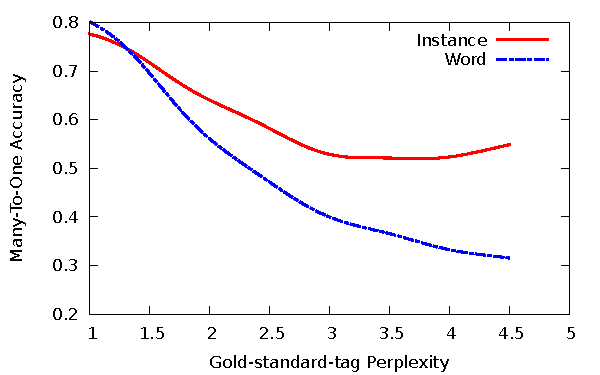
\includegraphics[width=.7\textwidth]{ksmooth-f.pdf} 
  \caption{The accuracy comparison of word and instance based
    part-of-speech induction models as a function of target word
    ambiguity (as measured by gold-standard-tag perplexity described
    in Section~\ref{sec:typevsinstance}) on the Penn Treebank.}
  \label{fig:perplexity}
\end{figure}

The obvious limitation of the one-tag-per-word assumption is that
instances of ambiguous words that have more than one POS role are
grouped into the same class.  For example, the word {\em offer} is
tagged as NN(399), VB(105) and VBP(34)\footnote{NN, VB and VBP are
  three POS tags from the Penn Treebank corpus and they correspond to
  singular noun, verb in base form and non-$3^{rd}$person singular
  verb in present tense, respectively.  The numbers in parentheses are
  the frequencies.} in its 538 occurrences in the human labeled Wall
Street Journal (WSJ) Section of the Penn Treebank (PTB) corpus
\cite{treebank3}.  If all instances of {\em offer} are assigned to the
most frequent tag NN, 36\% (139/538) will be erroneously labeled.  In
spite of this shortcoming, word-based POS induction systems generally
do well because the one-tag-per-word assumption is mostly accurate:
93.69\% of the word occurrences are tagged with their most frequent
POS tag in the PTB \cite{Toutanova:2003:FPT:1073445.1073478}.

In order to handle ambiguous words, models without a strict
one-tag-per-word assumption need to group word {\em instances} into
clusters according to their contexts.  Some of these instance-based
models bias words to have few tags using sparse priors in a Bayesian
setting
\cite{goldwater-griffiths:2007:ACLMain,johnson:2007:EMNLP-CoNLL2007,Gao:2008:CBE:1613715.1613761},
or posterior regularization \cite{Ganchev:2010:PRS:1859890.1859918}.
Sch\"{u}tze \shortcite{SchutzePe93} represents the context of a word
instance by concatenating context vectors of its left and right
neighboring words, and clusters word instances.  Berg-Kirkpatrick et
al.  \shortcite{bergkirkpatrick-klein:2010:ACL} use an EM algorithm
where they replace the multinomial components with miniature logistic
regressions and achieve the highest instance-based accuracy on PTB.
Christodoulopoulos et al.
\shortcite{Christodoulopoulos:2010:TDU:1870658.1870714} select
prototypes of each cluster from the output of Brown
\shortcite{Brown:1992:CNG:176313.176316} and feed them to a HMM model
that can handle prototypes as features
\cite{Haghighi:2006:PLS:1220835.1220876}.  However none of these
models achieve results comparable to the best word-based systems.  

In this work, we show that one can build an instance-based system that
can perform significantly better on highly ambiguous words (see
Figure~\ref{fig:perplexity}) and yet is competitive with word-based
systems in overall accuracy.

We follow the state of the art word-based system
\cite{yatbaz-sert-yuret:2012:EMNLP-CoNLL} and use probable substitutes
of a word instance as its contextual features.  The following examples
illustrate how such paradigmatic (substitute based) contextual
features can capture the similarity between two contexts where a
syntagmatic (neighbor based) representation would fail:

\begin{quotation}
(1) {\em ``Pierre Vinken, 61 years old, will join the board
  as a nonexecutive {\bf director} Nov.~29.''} 
\\ director $\rightarrow$ chairman
(.8242), director (.0127), directors (.0127) $\ldots$

(2) {\em ``$\ldots$ Joseph Corr was succeeded by Frank
  Lorenzo, {\bf chief} of parent Texas Air.''} 
\\ chief $\rightarrow$ chairman
(.9945), president (.0031), directors (.0012) $\ldots$
\end{quotation}

Each sentence has the target words marked in bold ({\bf director} and
{\bf chief}) and their likely substitutes listed with
probabilities\footnote{Substitute probabilities are computed using a
  4-gram language model.} in parentheses.  Note that the two contexts
have no words in common, therefore syntagmatic (neighbor based)
contextual features will fail to capture their similarity.  However,
paradigmatic features such as the top substitutes ``chairman'',
``directors'', etc.  clearly indicate the similarity and help place
these two instances into the same category.

Following \cite{globerson2007euclidean}, we embed words and their
contextual, orthographic, and morphological features in a high
dimensional Euclidean space that relates their joint probability to
distance.  In contrast to \cite{yatbaz-sert-yuret:2012:EMNLP-CoNLL} we
build an {\em instance-based} POS induction system where each instance
has a vector representation that concatenates the word vector with the
average of the contextual feature vectors.  We show that clustering of
these instance vectors separate different roles of ambiguous words
well, and achieve comparable or better performance than the best
word-based systems in matching the gold tags on 19 corpora in 15
languages.  All the code that can be used to replicate our findings is
available at \url{https://github.com/ai-ku/upos_2014}.

Section~\ref{sec:algorithm} describes the instance-based POS induction
algorithm, Section~\ref{sec:exp} gives the results of our experiments,
Section~\ref{sec:discuss} compares the output of the induction system
with the gold tags, and Section~\ref{sec:contrib} summarizes our
contributions.

%\section{Related Work}
\label{sec:related}
%%% This part looks fine
There are several good reviews of algorithms for unsupervised
part of speech induction
\cite{Christodoulopoulos:2010:TDU:1870658.1870714,Gao:2008:CBE:1613715.1613761}
and models of syntactic category acquisition \cite{ambridge2011child}.

This work is to be distinguished from supervised part of speech
disambiguation systems, which use labeled training data
\cite{Toutanova:2003:FPT:1073445.1073478}, unsupervised disambiguation
systems, which use a dictionary of possible tags for each word
\cite{yatbaz-yuret:2010:POSTERS}, or prototype driven systems
which use a small set of prototypes for each class
\cite{Haghighi:2006:PLS:1220835.1220876}.  The problem of induction is
important for studying under-resourced languages that lack labeled
corpora and high quality dictionaries.  It is also essential in
modeling child language acquisition because every child manages to
induce syntactic categories without access to labeled sentences,
labeled prototypes, or dictionary constraints.
%%%%
%\paragraph{Distributional vs. Feature Based}
% \subsection{Distributional vs. Feature Based}

Models of unsupervised part of speech induction fall into two broad groups
based on the usage of one-tag-per-word assumption.  Word type based models
enforce the one-tag-per-word solution.  Word instance based models can assign
instances of a word type to different POS clusters.

\subsection{Distributional models}

Distributional models can be further categorized into three subgroups
based on the learning algorithm.  The first subgroup represents each
word type/instance with its context vector and clusters these vectors
accordingly \cite{Schutze:1995:DPT:976973.976994}.  Work in modeling
child syntactic category acquisition has generally followed this
clustering approach
\cite{redington1998distributional,mintz2003frequent}.  The second
subgroup consists of probabilistic models based on the Hidden Markov
Model (HMM) framework \cite{Brown:1992:CNG:176313.176316}.  A third
group of algorithms constructs a low dimensional representation of the
data that represents the empirical co-occurrence statistics of word
types \cite{globerson2007euclidean}, which is covered in more detail
in Section~\ref{app:codethr}.

\paragraph{Clustering}
Clustering based methods represent the context using the neighboring
words, typically a single word on the left and a single word on the
right called a ``frame'' (e.g., {\em {\bf the} dog {\bf is}; {\bf the}
  cat {\bf is}}).  They cluster word types rather than word instances 
based on the frames they occupy thus employing one-tag-per-word
assumption from the beginning (with the exception of
\cite{mintz2003frequent,20674613} and some methods in
\cite{Schutze:1995:DPT:976973.976994}).  They may suffer from the data
sparsity caused by the infrequent words and the infrequent contexts.
The solutions suggested either restrict the set of words and set of
contexts to be clustered to the most frequently observed, or use
dimensionality reduction.  Redington et
al. \shortcite{redington1998distributional} define context similarity
based on the number of common frames bypassing the data sparsity
problem but achieve lower scores than the best performing systems.
Mintz \shortcite{mintz2003frequent} only uses the most frequent 45
frames to cluster instances and achieves 98\% unsupervised accuracy on
the instances observed in the most frequent 45 frames.  Similar to
Mintz's work, St Clair et al. \shortcite{20674613} show that systems
that model the left and right frames of instances seperately perform
better than the frequent frames both in terms of instances clustering
accuracy and the instances coverage.  Biemann
\shortcite{biemann2006unsupervised} contructs a graph based view of
the most frequent 10,000 words using contexts formed from the most
frequent 150-200 words and clusters the instances.  Sch\"utze
\shortcite{Schutze:1995:DPT:976973.976994} and Lamar et
al. \shortcite{lamar-EtAl:2010:Short} employ SVD to enhance similarity
between less frequently observed word types and contexts.  Lamar et
al. \shortcite{Lamar:2010:LCU:1870658.1870736} represent each context
by the currently assigned left and right tag (which eliminates data
sparsity) and cluster word types using a soft k-means style iterative
algorithm.  They report the best clustering result to date of .708
many-to-one accuracy on the PTB.
% all except schutze cluster word types

\paragraph{HMMs}
The prototypical bitag HMM model maximizes the likelihood of the
corpus $w_1 \ldots w_n$ expressed as $P(w_1|c_1)\prod_{i=2}^n
P(w_i|c_i) P(c_i|c_{i-1})$ where $w_i$ are the word instances and $c_i$
are their (hidden) tags.  One problem with such a model is its
tendency to distribute probabilities equally and the resulting
inability to model highly skewed word-tag distributions observed in
hand-labeled data \cite{johnson:2007:EMNLP-CoNLL2007}.  To favor
sparse word-tag distributions one can enforce a strict
one-tag-per-word solution (type clustering)
\cite{Brown:1992:CNG:176313.176316,Clark:2003:CDM:1067807.1067817},
use sparse priors in a Bayesian setting
\cite{goldwater-griffiths:2007:ACLMain,johnson:2007:EMNLP-CoNLL2007},
or use posterior regularization
\cite{Ganchev:2010:PRS:1859890.1859918}.  Each of these techniques
provide significant improvements over the standard HMM model: for
example Gao and Johnson \shortcite{Gao:2008:CBE:1613715.1613761} show
that sparse priors can gain from 4\% (.62 to .66 on the PTB) in
cross-validated many-to-one accuracy.  However Christodoulopoulos et
al. \shortcite{Christodoulopoulos:2010:TDU:1870658.1870714} show that
the older one-tag-per-word models such as
\cite{Brown:1992:CNG:176313.176316} outperform the more sophisticated
sparse prior and posterior regularization methods both in speed and
accuracy (the Brown model gets .68 many-to-one accuracy on the PTB).
Given that 93.69\% of the word occurrences in human labeled data are
tagged with their most frequent part of speech
\cite{Toutanova:2003:FPT:1073445.1073478}, this is probably not
surprising; one-tag-per-word is a fairly good first approximation for
induction.

%% \paragraph{Co-occurrence embedding}
%% Embedding algorithms maps the original data to a lower dimensional
%% space that preserves certain similarity structure defined between the
%% objects in the data.  However in real life problems such as POS
%% induction the similarity between contexts and word types can not be
%% trivially constructed given that only the co-occurrence information
%% exists between word types and their contexts.
%% S-Code\cite{NIPS2010_1196} which is a spherical extension of
%% \cite{Globerson:2007:EEC:1314498.1314572} algorithm maps the
%% word-types and their contexts on to a low dimensional Euclidean sphere
%% while preserving the co-occurrence statistics between them and then
%% clusters the low dimensional data with k-means algorithm.  They report
%% .688 many-to-one accuracy on PTB with 45 tags.

\subsection{Word-feature models}
One problem with the algorithms in the previous section is the poverty
of their input features.  Of the syntactic, semantic, and
morphological information linguists claim underlie syntactic categories,
context vectors or bitag HMMs only represent limited syntactic information in
their input.  Clark \shortcite{Clark:2003:CDM:1067807.1067817}, and Blunsom and
Cohn \shortcite{blunsom-cohn:2011:ACL-HLT2011} cluster types by incorporating
similar orthographic features and report improvements of 3 and 10\%
respectively over the baseline Brown model.  Berg-Kirkpatrick et al.
\shortcite{bergkirkpatrick-klein:2010:ACL} incorporate orthographic features
into EM algorithm where they replace the multinomial components with miniature
logistic regressions and cluster instances while improving the Brown model by 7\%.

Christodoulopoulos et
al. \shortcite{Christodoulopoulos:2010:TDU:1870658.1870714} use
prototype based features as described in
\cite{Haghighi:2006:PLS:1220835.1220876} with automatically induced
prototypes and report an 8\% improvement over the baseline Brown model
by clustering instances.  Abend et
al. \shortcite{Abend:2010:IUP:1858681.1858813} train a
prototype-driven model with morphological features by first clustering
the high frequent types as the landmarks and then assigning the
remaining types to these landmark clusters.  Christodoulopoulos et
al. \shortcite{christodoulopoulos-goldwater-steedman:2011:EMNLP}
define a type-based Bayesian multinomial mixture model in which each
word instance is generated from the corresponding word type mixture
component and word contexts are represented as features.  They achieve
a .728\ \mto\ score by extending their model with additional
morphological and alignment features gathered from parallel corpora.
To our knowledge, nobody has yet tried to incorporate phonological or
prosodic features in a computational model for syntactic category
acquisition.

\subsection{Paradigmatic representations}

Yatbaz et al. \shortcite{yatbaz-sert-yuret:2012:EMNLP-CoNLL} explore
the paradigmatic representation of the word contexts by modeling the
co-occurrence of words and their substitutes within the S-CODE
framework.  Their experiments on the PTB types shows that paradigmatic
representation improves the state-of-the-art \mto\ and V-measure (\vm)
accuracies of both distributional models and models with additional
word features.  This paper builds on that preliminary work by
%% (1) exploring clustering of substitute vectors,
(1) exploring induction of part-of-speechs at instances level (in addition
to type level), (2) improving the model for using additional features,
and (3) experimenting with additional languages.


%% This paper defines a new representation that models the features from
%% different domains as separate variables and relates them to each other
%% by using their co-occurrence statistics with a shared variable
%% (i.e. word types).

\subsection{Evaluation}
%% It is natural to question the merit of evaluating unsupervised results
%% by comparing them to gold standard tags.  For example
%% \cite{freudenthal2005resolution} argue that a verb category (such as
%% {\sc vb} in Penn Treebank) that contains verbs that can and cannot be
%% used in certain constructions (e.g. the imperative) and verbs that can
%% be used as both auxiliaries and main verbs (e.g., {\em do, have}) does
%% not in fact constitute a set of items that could be substituted for
%% one another in particular sentences.  Such a category fails the
%% standard linguistic definition of a syntactic category and children do
%% not seem to make errors of substituting such words in utterances
%% (e.g. {\em''What do you want?''} vs. {\em *''What put you want?''}).
%% They suggest evaluating models by incorporating a production component
%% that allows the model's output to be compared to speech produced by
%% children exposed to the same input.  \cite{frank2009evaluating},
%% motivated by the lack of gold standards for many novel languages,
%% suggest comparing a system's clusters to a set of clusters created
%% from {\em substitutable frames}.  They create frames using two words
%% appearing in the corpus with exactly one word between and calculate
%% precision, recall, and F-score of the system's clustering.
%% Statistical parsers or factored machine learning systems could also be
%% sources of extrinsic evaluation for induced syntactic categories.  We
%% hope such extrinsic evaluation will be more widespread in the future
%% but nevertheless use many-to-one (\mto) and V-measure (\vm) metric on
%% the 45-tag Penn Treebank gold standard to evaluate the current work.

We report many-to-one and V-measure scores for our experiments as
suggested in \cite{Christodoulopoulos:2010:TDU:1870658.1870714}.  The
many-to-one (\mto) evaluation maps each cluster to its most frequent
gold tag and reports the percentage of correctly tagged instances.
The \mto\ score naturally gets higher with increasing number of
clusters but it is an intuitive metric when comparing results with the
same number of clusters.  The V-measure (\vm) \cite{rosenberg2007v} is
an information theoretic metric that reports the harmonic mean of
homogeneity (each cluster should contain only instances of a single
class) and completeness (all instances of a class should be members of
the same cluster).  In Section~\ref{sec:discuss} we argue that
homogeneity is perhaps more important in part of speech induction and
suggest \mto\ with a fixed number of clusters as a more intuitive
metric.

%% \paragraph{Many-to-one (MTO)} metric measures the cluster purity 
%% therefore each cluster is mapped to the most frequent gold tag of the
%% words observed in that cluster.  \mto metric is the most intuitive
%% measure, however it has a bias towards to the increasing number of
%% clusters thus it should be used when the number of clusters is fixed
%% \cite{christodoulopoulos-goldwater-steedman:2011:EMNLP}.
%% \paragraph{V-measure (VM)} is an entropy based metric that calculates
%% weighted average of cluster homogeneity and completeness in a similar
%% fashion with F-measure recall and precision, respectively.  The
%% cluster homogeneity is an analogy of the cluster purity in \mto.
%% Although \vm is more robust to variable number of clusters, it is less
%% intuitive than \mto
%% \cite{christodoulopoulos-goldwater-steedman:2011:EMNLP}.  Moreover it
%% punishes the clustering when words with same gold tag distributed over
%% different clusters which contradicts with the idea of POS induction
%% since the aim is to cluster words according to the underlying natural
%% grouping.

%%% DY: where is the original paper that introduced V-measure?
%%% DY: are you sure Chris2011 is the right citation, shouldn't it be Chris2010?


\section{Algorithm}
\label{sec:algorithm}

In this section, we describe the steps of our instance-based
POS-induction algorithm:
\begin{enumerate}
  \item Sample $r$ substitutes for each word instance in the target
    corpus using an n-gram language model.
  \item Construct $r$ tuples for each instance where each tuple
    consists of a sampled substitute, the target word, and the
    morphological and orthographical features of the target word.
  \item Construct Euclidean embeddings of each word and each feature based on
    all tuples following Gleberson et al.\shortcite{globerson2007euclidean}
    and Maron et al.\shortcite{maron2010sphere}.
  \item Construct a vector representation for each instance by
    concatenating the embedding of the target word with the average of
    its substitute embeddings.
  \item Use $k$-means clustering to cluster the instance vectors where
    $k$ is equal to the number of gold tags.
  \item Construct a mapping from clusters to tags for evaluation using
    the most frequent tag found in each cluster.
\end{enumerate}

Steps 1 and 2 construct a tuple representation for each instance.
Table~\ref{tab:sampleswithfeatures} gives some example tuples for Sentence (1)
from the previous section.  In this example $r=3$, so three substitutes are
sampled for each instance as contextual features.  The sampling is with
replacement from the substitute word distribution of a given context using the
n-gram language model, so some substitute words may be repeated.  The target
word and its other features are identical for each of the $r$ tuples
representing a single instance.

\begin{table}[h]
  \centering
  \begin{tabular}{|lllll|}
    \hline
    {\bf Word} & {\bf Subst} & {\bf Suf} & {\bf Cap} & {\bf Num} \\
    \hline
    Vinken & Makhlouf & -- & T & F\\
    Vinken & Makhlouf & -- & T & F\\
    Vinken & \unk & -- & T & F\\
    61 & 20 & -- & F & T\\
    61 & 2000 & -- & F & T\\
    61 & eleven & -- & F & T\\
    years & years & -s & F & F\\
    years & years & -s & F & F\\
    years & years & -s & F & F\\
    \hline
  \end{tabular}
  \caption{The tuples constructed for the instances of ``Vinken'',
    ``61'' and ``years'' from Sentence (1).  The elements of each tuple
    are the target word, sampled substitute, suffix, capitalization, and
  the presence of numeric characters.}
  \label{tab:sampleswithfeatures}
\end{table}

%% We construct the co-occurrence data as word--features tuples that consist of
%% word, and its contextual (substitutes), orthographic and morphological
%% features.  Contextual features are sampled from the substitute word
%% distribution of the instance context.  If $r$ random substitutes are sample for
%% each instance than there will be $r$ identical tuples except the contextual
%% features.  Table~\ref{tab:sampleswithfeatures} presents the co-occurrence
%% tuples of each instance in a sample sentence when $r$ is equal to 1.  

%% \begin{table*}[!t]
%%   \centering
%%   \footnotesize
%% \begin{tabular}{|lllllll|}
%%   \hline
%%   \textbf{Word} & {\bf Contextual} & {\bf Morphology} &
%%   \specialcell{{\bf Initial}\\{\bf Capital}} & {\bf Number} &
%%   \specialcell{{\bf Contains}\\{\bf Hypen}} &
%%   \specialcell{{\bf Initial}\\{\bf Apostrophe}}
%%   \\
%%   \hline
%%   W:Pierre & \textit{C:Adrian} & & {\it F:IC} &&&\\
%%   W:Vinken & \textit{C:Danon} & & {\it F:IC} &&&\\
%%   W:, & \textit{C:\{} & & &&&\\
%%   W:61 & \textit{C:fourteen} & & & {\it F:N}&&\\
%%   W:years & \textit{C:years} & {\it F:s} &&&&\\
%% %%W:old & \textit{C:old} & & &&&\\
%% %%W:join & \textit{C:head} &&&&&\\
%% %%W:the & \textit{C:its} &&&&&\\
%% %%W:board & \textit{C:company} &&&&&\\
%% %%W:as & \textit{C:as} &&&&&\\
%% %%W:a & \textit{C:a} &&&&&\\
%% %%W:nonexecutive & \textit{C:non-executive} &&&&&\\
%% %%W:director & \textit{C:chairman} & {\it F:or}&&&&\\
%% %%W:Nov. & \textit{C:May} &&{\it F:IC}&&&\\
%% %%W:29 & \textit{C:9} &&&{\it F:N}&&\\
%% %%W. & \textit{C:.} & &&&&\\
%%   \hline
%% \end{tabular}
%% \caption{The first five words of the input sentence \textit{``Pierre Vinken, 61
%%   years old, will join the board as a nonexecutive director Nov.~29 .''} is
%%   represented with their contextual, orthographic and morphological features as
%%   tuples.  The leftmost column presents the target word, second column
%%   represents the contextual, third column is the morphological and the rest of
%%   the columns are the orthographic features.  Unobserved features are set to
%%   null.}
%% \label{tab:sampleswithfeatures}
%% \end{table*}

In step 3, we construct Euclidean embeddings for each unique word and feature
value using the multi-variable version of the CODE algorithm described in
\cite{globerson2007euclidean}, Section 6.2.  The CODE algorithm models the
pairwise joint distributions between target words and their contextual,
morphological, and orthographic features by embedding the frequently
co-occuring pairs closer in Euclidean space.  The spherical optimization
(S-CODE) described in \cite{maron2010sphere} is used for efficiency.
Appendix~A details the model likelihood and the training procedure in our
setup. 

%% To handle co-occurrence tuples we use the modified version of S-CODE that can
%% model more than two variables (see Appendix~\ref{app:multiscode}).  We feed
%% the tuples to the modified S-CODE which places $n$-dimensional embeddings for
%% word types that frequently co-occur with the same features (and features that
%% co-occur with the same words types) close to each other on the sphere.
%% Figure~\ref{fig:scodeexample} illustrates the embeddings of a sample
%% co-occurrence data on a sphere after S-CODE converges.  This modified S-CODE is
%% aware of the feature types which enables us to construct our instance based
%% representation.  In addition, the modified S-CODE can weight the different
%% feature types and this will be the interest of future work. 

%% \begin{figure}[h]
%% \centering
%%  \begin{minipage}[c]{0.49\columnwidth}
%%   \footnotesize
%%   \begin{tabular}{l|l}
%%     \textbf{Word} & \textbf{Substitute} \\
%%     \hline
%%     $\hdots$&$\hdots$\\
%%     W:director & S:chairman \\
%%     W:chief & S:chairman \\
%%     $\hdots$&$\hdots$\\
%%     W:Pierre & S:John \\
%%     W:Frank & S:John \\
%%     $\hdots$&$\hdots$\\
%%   \end{tabular}
%%   \end{minipage} \hfill
%%   \begin{minipage}[c]{0.49\columnwidth}
%%     \raisebox{-\height}{
%%       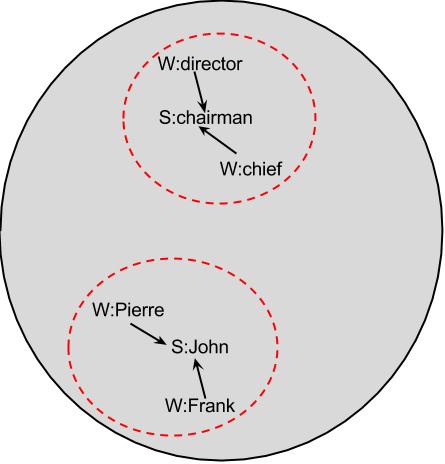
\includegraphics[width=1\columnwidth]{scode-ex.png}
%%     }
%%   \end{minipage}
%%   \caption{The table on the left is a co-occurrence data and  figure on the
%%   right represents the final embeddings of the words and contextual features
%%   after S-CODE converges.  Dashed circles represent the possible groupings of the
%%   word type embeddings on the sphere.}
%%   \label{fig:scodeexample}
%% \end{figure}

%The limitation of representing co-occurrence data as pairs is that S-CODE can
%not distinguish whether the type of the word-feature pair is contextual,
%orthographic or morphological.  

Step 4 constructs a vector representation for each word instance with the
concatenation of its word type embedding and the average of its $r$ substitute
embeddings.  If the original embeddings are in $d$ dimensional space, this
results in a $2d$ dimensional vector representing an instance.  Step 5 clusters
these $2d$ dimensional instance vectors using a modified k-means algorithm with
smart initialization \cite{arthur2007k} and assigns each instance to one of $k$
clusters.  Step 6 constructs a mapping between the clusters and the gold tags
for evaluation.  

%% Yatbaz et al.\shortcite{yatbaz-sert-yuret:2012:EMNLP-CoNLL} model co-occurrence
%% pairs using the S-CODE with two variables and cluster the embeddings of word
%% types with weighted k-means algorithm.  The sentences in
%% Figure~\ref{fig:typelimitation} illustrates the limitation of clustering word
%% type embeddings.  The word {\em offer} is a {\em verb} in the first sentence
%% and a {\em noun} in the second one.  S-CODE constructs only one embedding for
%% each unique word type and feature value.  Thus clustering the word type
%% embeddings is actually applying the one-tag-per-word assumption.

%% \begin{figure}[ht]
%%   %  \begin{minipage}[c]{\columnwidth}
%%     \begin{tabular}{ll}
%%       (1) & $\hdots$ it will also {\em offer} buyers the option $\hdots$\\
%%       &{\bf Substitutes:} give, help, attract\\ 
%%       (2) & The {\em offer} is being launched $\hdots$\\ 
%%       &{\bf Substitutes:} campaign, project, scheme\\ 
%%     \end{tabular}
%%    \caption{Ambiguous occurrences of the word {\em offer}.}
%%    \label{fig:typelimitation}
%%    %\end{minipage} \hfill
%%  \end{figure}
%% On the other hand, the substitutes of {\em offer} in both of the sentences can
%% semantically and syntacticly disambiguates the correct category of the
%% corresponding occurrences.  

%% The next section presents the results of our system and compares them with the
%% results of the word based state-of-the-art system. 
%% To construct the co-occurrence data we pair each word instance with randomly
%% sampled substitutes that can be observed in the context of the corresponding
%% instance and with orthographic and morphological features of the word instance.
%% Random substitutes were sampled (with replacement) from a substitute word
%% distribution for the context calculated based on an n-gram language model.  
%% 
%% We enriched the word--substitute co-occurrence data by extracting morphological
%% and orthographic features and incorporating them as word--feature pairs.  They
%% fed the co-occurrence data into the S-CODE algorithm.  S-CODE places the
%% embeddings for word types that frequently co-occur with the same substitutes or
%% features (and substitutes or features that co-occur with the same words) close
%% to each other on the $n$-dimensional sphere.  Finally, they apply k-means
%% clustering to group vectors of word types to induce word categories.
%% 
%% First, we construct a pairwise co-occurrence
%% representation of words and their substitutes.  Next, we map each word and each
%% substitute in the co-occurrence data to real vectors (embeddings) on an
%% $n$-dimensional sphere using the S-CODE algorithm \cite{maron2010sphere}.
%% S-CODE places the vectors for words that frequently co-occur with the same
%% substitutes (and substitutes that co-occur with the same words) close to each
%% other on the sphere.  We then construct vectors for each word instance by using
%% the embeddings of the word itself and its sampled substitutes in the
%% co-occurrence data.  Finally, we apply k-means clustering to group these
%% vectors to induce word categories.  
%% 
%% In Section~\ref{sec:cooc} we detail the representation of words and their
%% substitutes as co-occurrence data, in Section~\ref{sec:embedding} we describe
%% the embedding algorithm, and finally Section~\ref{sec:clustering} describes how
%% we represent the word instances using the embeddings calculate in the previous
%% step.
%% 
%% \subsection{Context Representation}
%% \label{sec:cooc}
%% % How we represent the context?
%% % How we relate the word and the context?
%% 
%% We represent the context of a word with random substitutes that are
%% likely to occupy the same position as the word.  We sample random
%% substitutes (with replacement) from a substitute word distribution for
%% the context calculated based on an n-gram language model.  The sample
%% space of the substitute word distribution is the vocabulary of the
%% language model.
%% %% \footnote{Sampled substitutes might include the unknown
%% %%   word tag \unk\ representing words outside the fixed size
%% %%   vocabulary of the language model.  For example proper nouns
%% %%   typically have \unk\ as a substitute.}  
%% In effect, we are using substitute word distributions and the sampled random
%% substitutes as {\em contextual features} that represent properties of a word's
%% position.  Table~\ref{tab:subdist} shows the substitute word distributions for
%% some positions in an example sentence.
%% %% \begin{table*}[t]
%% %%   \footnotesize
%% %%   \centering
%% %%   \caption{The substitute word distributions (with probabilities in
%% %%     parentheses) for some of the positions in the example sentence
%% %%     \textit{``Pierre Vinken, 61 years old, will join the board as a
%% %%     nonexecutive director Nov.~29.''} based on a 4-gram language
%% %%   model.}
%% %%   \label{tab:subdist}
%% %%   \begin{tabular}{|ll|} \hline
%% %%     \textbf{will:} & \textit{will} (0.9985), \textit{would} (0.0007), \textit{to} (0.0006), \textit{also} (0.0001), $\ldots$ \\
%% %%     \textbf{join:} & \textit{join} (0.6528), \textit{leave} (0.2140), \textit{oversee} (0.0559), \textit{head} (0.0262), \textit{rejoin} (0.0074), $\ldots$ \\
%% %%     \textbf{the:}  &\textit{its} (0.9011), \textit{the} (0.0981), \textit{a} (0.0006), $\ldots$ \\
%% %%     \textbf{board:} & \textit{board} (0.4288), \textit{company} (0.2584), \textit{firm} (0.2024), \textit{bank} (0.0731), \textit{strike} (0.0030), $\ldots$ \\
%% %%     \hline
%% %%   \end{tabular}
%% %% \end{table*}
%% %%
%% To capture the relation between each word and its context we construct
%% a co-occurrence representation by pairing the words with randomly
%% sampled substitutes.  Table~\ref{tab:samples} shows random substitutes of each
%% word and their pairwise co-occurrence representation input to S-CODE on an
%% example sentence.  It is possible (and beneficial) to sample more than one
%% substitute and generate multiple pairs for the same word-context pair as seen
%% in Table~\ref{tab:samples}.  In the co-occurrence data, a target word might
%% appear both as a word and a random substitute therefore to clarify this
%% ambiguity we prepend ``W:'' and ``S:'' to words and substitutes, respectively.
%% The calculation of substitute distributions and substitute word sampling are
%% detailed in Appendix~A.
%% %% \begin{table}[h]
%% %%   \footnotesize
%% %%   \caption{The table on the left shows three possible substitutes
%% %%     sampled with replacement for each position in an example sentence
%% %%     based on a 4-gram language model.  The table on the right is the
%% %%     pairwise co-occurrence data fed to the S-CODE algorithm derived
%% %%     from these samples.  The prefixes ``W:'' and ``S:'' are used to
%% %%     distinguish target words and substitutes.  Sampled substitutes
%% %%     might include the unknown word tag ``\unk'' representing words
%% %%     outside the fixed size vocabulary of the language model.}
%% %% \begin{tabular}{|ll|} \hline
%% %% \textbf{Word} & \textbf{Random Substitutes}\\
%% %% \hline
%% %% Pierre & \textit{Mr.}  / \textit{Pierre} /  \textit{John}\\
%% %% Vinken & \textit{\unk} / \textit{Beregovoy} / \textit{Cardin}\\
%% %% %, & \textit{,} / \textit{,} / \textit{,}\\
%% %% %61 & \textit{48} / \textit{52} / \textit{41}\\
%% %% %years & \textit{years} /  \textit{years} /  \textit{years}\\
%% %% %old & \textit{old} /  \textit{old} /  \textit{old}\\
%% %% %, & \textit{,} /  \textit{,} /  \textit{,}\\
%% %% %will & \textit{will} /  \textit{will} /  \textit{will}\\
%% %% $\hdots$&\\
%% %% join & \textit{head} /  \textit{join} /  \textit{leave}\\
%% %% the  & \textit{its} /  \textit{its} /  \textit{the}\\
%% %% %board & \textit{board} /  \textit{company} / \textit{firm}\\
%% %% $\hdots$&\\
%% %% %as & \textit{as} / \textit{as} / \textit{as}\\
%% %% %a & \textit{a} / \textit{a} / \textit{a}\\
%% %% %nonexecutive & \textit{nonexecutive} / \textit{non-executive} / \textit{nonexecutive}\\
%% %% $\hdots$&\\
%% %% director & \textit{chairman} / \textit{chairman} / \textit{director}\\
%% %% $\hdots$&\\
%% %% %Nov. & \textit{April} / \textit{May} / \textit{of}\\
%% %% %29 & \textit{16} /  \textit{29} / \textit{9}\\
%% %% %. & \textit{.}  / \textit{.} / \textit{.}\\
%% %% \hline
%% %% \end{tabular}
%% %% \quad
%% %% \begin{tabular}{|ll|}
%% %% \hline
%% %% \textbf{Word} & \textbf{Substitute}\\
%% %% \hline
%% %% W:Pierre & \textit{S:Mr.}\\
%% %% W:Pierre & \textit{S:Pierre}\\
%% %% W:Pierre & \textit{S:John}\\
%% %% W:Vinken & \textit{S:\unk}\\
%% %% W:Vinken & \textit{S:Beregovoy}\\
%% %% W:Vinken & \textit{S:Cardin}\\
%% %% $\hdots$&\\
%% %% W:join & \textit{S:head}\\
%% %% W:join & \textit{S:join}\\
%% %% W:join & \textit{S:leave}\\
%% %% W:the & \textit{S:its}\\
%% %% W:the & \textit{S:its}\\
%% %% W:the & \textit{S:the}\\
%% %% $\hdots$&\\
%% %% W:director & \textit{S:chairman}\\
%% %% W:director & \textit{S:chairman}\\
%% %% W:director & \textit{S:director}\\
%% %% $\hdots$&\\
%% %% \hline
%% %% \end{tabular}
%% %% \label{tab:samples}
%% %% \end{table}
%% 
%% The next section describes the S-CODE algorithm which takes the
%% pairwise co-occurrence data as its input and calculates the embeddings
%% of the words and their substitutes on an $n$-dimensional sphere.
%% 
%% \subsection{Co-occurrence Embedding}
%% \label{sec:embedding}
%% The S-CODE algorithm maps each unique word and substitute in the
%% co-occurrence data to a real vector (embedding) on an $n$-dimensional
%% sphere as detailed in Appendix~B.  The basic idea of the mapping is
%% that words and substitutes that are frequently observed as pairs in
%% the co-occurrence data will have close embeddings while pairs
%% not observed together will have embeddings that are far apart from each
%% other.
%% 
%% %%   \begin{minipage}[c]{0.28\columnwidth}
%% %%     \footnotesize
%% %%     \begin{tabular}{l|l}
%% %%       \textbf{Word} & \textbf{Substitute} \\
%% %%       \hline
%% %%       $\hdots$&$\hdots$\\
%% %%       W:offer & S:give\\
%% %%       W:offer & S:help\\
%% %%       W:offer & S:attract\\
%% %%       W:offer & S:campaign\\
%% %%       W:offer & S:project\\
%% %%       W:offer & S:scheme\\
%% %%       $\hdots$&$\hdots$\\
%% %%     \end{tabular}
%% %%   \end{minipage} \hfill
%% %%   
%% %%  \begin{minipage}[c]{\columnwidth}
%% %%     \raisebox{-\height}{
%% %%       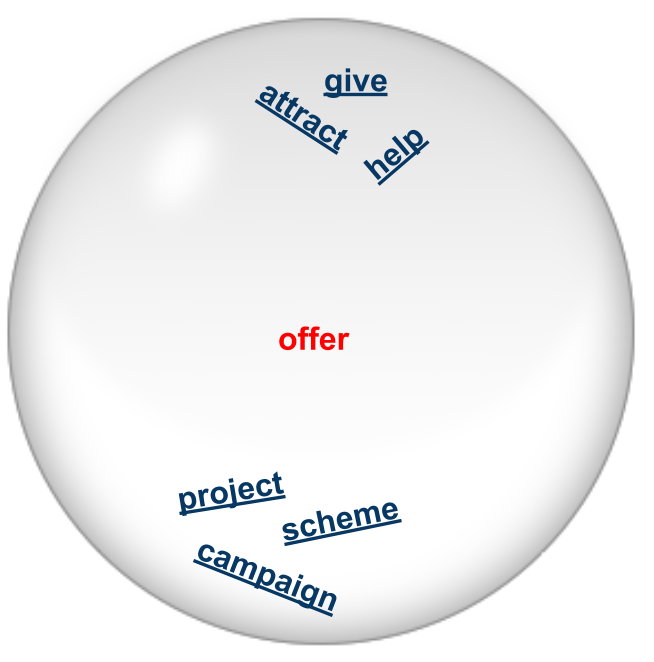
\includegraphics[width=0.5\columnwidth]{sphere.png}
%% %%     }
%% %%   \end{minipage}
%% %%   \caption{The figure on the left presents the input sentences and the randomly
%% %%     sampled substitutes of the word {\em offer} in each sentences.   The right
%% %%   one presents the final embeddings on a representative sphere after S-CODE
%% %%   converges.}
%% %%   \label{fig:scodeexample}
%% %% \end{figure}
%% 
%% The co-occurrence data in Figure~\ref{fig:scodeexample} consists of
%% pairs such as (\textit{W:director}, \textit{S:chairman}) and
%% (\textit{W:chief}, \textit{S:chairman}) therefore S-CODE forces the
%% embeddings of \textit{W:director} and \textit{W:chief} to be close to
%% the embedding of \textit{S:chairman}.  Similarly the embeddings of
%% \textit{W:Pierre} and \textit{W:Frank} will be close to the embedding
%% of \textit{S:John} because they are frequently co-occurring pairs.  As
%% a result the final embeddings of \textit{W:director} and
%% \textit{W:chief} will be close to each other due to the common
%% substitute \textit{S:chairman} and will be apart from
%% \textit{W:Pierre} and \textit{W:Frank} due to the lack of common
%% substitutes (similarly the embeddings of \textit{W:Pierre} and
%% \textit{W:Frank} will be close to each other due to \textit{S:John}).
%% 
%% The coordinates of the embeddings for each unique word and substitute
%% constitute the input to the clustering stage as described in the next
%% subsection.
%% 
%% % How we relate final embeddings and the input pairs?
%% %% S-CODE constructs embeddings on an $n$-dimensional sphere for each word
%% %% type and substitute.  Each pair in the co-occurrence data can be
%% %% represented in three different ways by using the output of S-CODE: (1)
%% %% word embedding (${\bf W}$) which represents the word type information,
%% %% (2) substitute embedding (${\bf C}$) which represents the context
%% %% information, and (3) concatenation of word and substitute embeddings
%% %% (${\bf W}\oplus{\bf C}$).  In the next section we apply k-means
%% %% clustering to these three representation and analyze the
%% %% characteristic of final clusters.
%% 
%% \subsection{Clustering}
%% \label{sec:clustering}
%% %% In Section~\ref{sec:cooc} we describe the transformation of an input
%% %% sentence to a co-occurrence data and we represent each target word
%% %% with the word--substitute pair(s).  In the previous section we
%% %% construct embeddings for each value observed in the co-occurrence data
%% %% using the S-CODE algorithm. 
%% 
%% At this stage, each unique word in the text and each unique substitute
%% sampled to represent their contexts is mapped to a real vector
%% embedding on an $n$ dimensional sphere\footnote{In fact many words
%%   that appear in the text also appear as substitutes and thus get two
%%   embeddings.}.  We apply the instance weighted k-means clustering
%% algorithm to three different representations derived from these
%% embeddings, each with its own advantages and disadvantages:
%% 
%% \paragraph{Type Based:} 
%% In this clustering, each target word {\em type} has a single embedding, and gets
%% assigned to a single cluster.  Clustering word embeddings was previously
%% explored in \cite{yatbaz-sert-yuret:2012:EMNLP-CoNLL}, which achieved the best
%% results to date (80\% \mto) for English.  Sections~\ref{sec:typevsinstance}
%% summarize these experiments for completeness.  
%% %% \paragraph{Clustering substitute embeddings (${\bf S}$)}  
%% %% In a second set of experiments, we ignore target word embeddings and
%% %% apply clustering only to substitute embeddings, associating each
%% %% substitute with a unique cluster.  We then categorize target word {\em
%% %%   tokens} based on what cluster the majority of their substitutes
%% %% belong.  It is important to note that in this setting we are ignoring
%% %% the identity and features of the target words and in effect clustering
%% %% word contexts (substitutes are determined by the context and are
%% %% conditionally independent of the target word).
%% %% 
%% %% For example, the target word {\it W:board} in Table~\ref{tab:samples}
%% %% will be represented with the embeddings of {\it S:board}, {\it
%% %%   S:company} and {\it S:firm} while another occurrence of the word
%% %% {\it W:board} in a different context might be represented with
%% %% embeddings of different substitutes such as {\it S:embark} or {\it
%% %%   S:enter}.  Each occurrence of the target word ``board'' is assigned
%% %% to the cluster in which the majority of its substitute embeddings are
%% %% present\footnote{Ties are broken randomly.}.  This approach generally
%% %% results in higher accuracy for highly ambiguous words like {\em offer}
%% %% where clustering substitute embeddings achieves .82 \mto\ compared
%% %% to the one-tag-per-word upper bound of .74.
%% %% Section~\ref{sec:clustering-s} presents the results of experiments
%% %% clustering substitute embeddings.
%% %% 
%% %% Unfortunately such highly ambiguous words do not constitute a
%% %% significant portion of the corpus and the overall accuracy suffers
%% %% (.64 compared to .80 \mto\ for word clustering).  We also observed
%% %% similar results in our preliminary experiments without S-CODE trying
%% %% to cluster contexts directly (using the Kullback-Leibler divergence
%% %% between their substitute distributions).  Many common words that occur
%% %% in similar contexts and that have similar substitutes, e.g. {\em his}
%% %% and {\em the}, belong to different parts of speech.  In addition,
%% %% words that are generally not substitutable like ``do'' and ``put'' are
%% %% placed in the same category by the PTB.  This suggests that the
%% %% identity and features of the target word are indispensable and that a
%% %% purely substitutability based linguistic definition is insufficient
%% %% for inducing parts of speech as tagged in the PTB.
%% 
%% \paragraph{Instance Based:}
%% In this clustering, we represent each word instance by concatenating the type
%% embedding ($n$ dimensional) with the average of substitutes of that particular
%% instance ($n$ dimensional).  We then apply k-means to the resulting
%% $2n$-dimensional vectors and categorize each instance of a type separately.
%% For instance, the target word ``Pierre'' in Table~\ref{tab:samples} will be
%% represented by concatenating the embedding of {\it W:Pierre} with the average
%% of the embeddings of {\it S:Mr.}, {\it S:Pierre} and {\it S:John}.  This model
%% do not employ the one-tag-per-word assumption and clusters word instances
%% therefore it handles ambiguity.  Clusters that are constructed according to
%% this representation tend to assign fewer categories to each word type than
%% substitute clustering due to the concatenation of ${\bf W}$.  The advantage in
%% highly ambiguous words is still retained (e.g. the \mto\ for {\em offer} is
%% .XX) and the overall result is comparable compared to clustering of word
%% embeddings.  Section~\ref{sec:instance} presents results of the instance based  
%% clustering.
%% 
%% \paragraph{Summary} The first clustering applies the one-tag-per-word
%% assumption from the beginning and clusters word types instead of instances. 
%% %The second setting clusters word contexts (as represented by
%% %substitutes) and is able to categorize individual word tokens.
%% %However it ignores the identity of the target word.  
%% The second one clusters word instances by representing each instance with the
%% concatenation of the word type and average of corresponding substitute
%% embeddings.  The target word is represented without enforcing the
%% one-tag-per-word assumption improves the results on highly ambiguous words
%% while achieving close results with the state-of-the-art system.
%% Section~\ref{sec:exp} compares the performance of these two clustering on the
%% part of speech induction problem, as well as
%% experiments with different features and languages.

\section{Experiments}
\label{sec:exp}

In this section we present our instance-based POS induction
experiments.  Section~\ref{sec:evaluation} describes the accuracy
metrics that we use to evaluate our results.  Section~\ref{sec:expset}
details the test corpus and the experimental parameters used in the
English experiments and compares our results with previous work.  
%% Section~\ref{sec:instance} presents the
%% performance of our instance based model on English POS induction and
%% performs sensitivity analysis.  
Section~\ref{sec:typevsinstance}
compares the performance of type and instance based systems on
ambiguous words.  Finally, Section~\ref{sec:multilang} extends the
language and corpus coverage by applying the best performing instance
based models to 19 corpora in 15 languages.

%% Clustering results on word types, first presented in
%% \cite{yatbaz-sert-yuret:2012:EMNLP-CoNLL}, are still state of the art for
%% English POS induction.  However in this study we show that the performance on
%% ambiguous words can be further improved by clustering word instances. 
%% (Sections~\ref{sec:clustering-s} and \ref{sec:clustering-c}), we improve the
%% model that incorporates morphological and orthographic features
%% (Section~\ref{sec:feat} and Appendix~C), and we demonstrate the applicability
%% of our methods to other languages (Section~\ref{sec:multilang}).
\subsection{Evaluation}
\label{sec:evaluation}
We report many-to-one and V-measure scores for our experiments as
suggested in \cite{Christodoulopoulos:2010:TDU:1870658.1870714}.  The
many-to-one (\mto) evaluation maps each cluster to its most frequent
gold tag and reports the percentage of correctly tagged instances.
The \mto\ score can be increased by simply increasing number of
clusters, thus the number of clusters is fixed to match the number of
gold tags in each experiment.  The V-measure (\vm)
\cite{rosenberg2007v} is an information theory motivated metric that
calculates the harmonic mean of completeness and homogeneity of the
clusters.  Completeness of a cluster is maximized when all instances
of a gold-tag are grouped into the same cluster and the homogeneity is
maximized when the members of a cluster belong to the same gold-tag.
%% In Section~\ref{sec:discuss} we argue that
%% homogeneity is perhaps more important in part of speech induction and
%% suggest \mto\ with a fixed number of clusters as a more intuitive
%% metric.

\subsection{Experimental Settings and Results}
\label{sec:expset}

To make a direct comparison with previously published results,
% what is the test data
the Wall Street Journal Section of the Penn Treebank was used as the
test corpus (1,173,766 instances, 49,206 unique tokens) for English
experiments.
% what is the tag set
PTB uses 45 part-of-speech tags which we used as the gold standard for
evaluation in our experiments.

% what is the LM training data
%Train => 88214605 2303225131 12630027619
To compute substitutes in a given context we trained a language model
using the ukWaC corpus ($\approx$ 2 billion tokens) constructed by
crawling the ``.uk'' Internet
domain \cite{ferraresi2008introducing}\footnote{We use the Penn
  Treebank Tokenizer to make the training data compatible with PTB.}.
% how is the language model trained
We used SRILM \cite{Stolcke2002} to build a 4-gram language model with
interpolated Kneser-Ney discounting.
% what is the vocabulary
Words that were observed less than 2 times in the language model
training data were replaced by \unk\ tags, which gave us a
vocabulary size of 4,254,946. 
% what is the test data
% perplexity
The perplexity of the 4-gram language model on the PTB is 303 and the
unknown word rate is 0.008.  For computational efficiency only the top
100 substitutes and their probabilities were computed for each
position in the PTB using the {\sc fastsubs} algorithm \cite{yuret2012fastsub}.  
% (1,173,766 instances, 49,206 types)
%% The probability vectors for each position were normalized to add up to
%% 1.0 giving us the final substitute distributions used in our
%% experiments.
We use the same orthographic features defined in
\cite{yatbaz-sert-yuret:2012:EMNLP-CoNLL} and generated morphological
features using the unsupervised algorithm Morfessor \cite{creutz05}.
%% Morfessor was trained on PTB using default settings, and a perplexity
%% threshold of 300.  We concern only the splits tagged as {\em suffix}
%% in the Morfessor output and allow at most one morphological feature
%% per word type \footnote{Splits are concatenated if there are
%%   consecutive suffix parts at the end of a word type.}.

%TODO: define phi_0, nu_0 in appendix.
% To make a meaningful comparison on the PTB
The experiments were run using the following default settings (unless otherwise
stated): (1) each word was kept with its original capitalization; (2) 90
substitutes sampled per instance; (3) the learning rate parameters for S-CODE
were set to $\varphi_0=50$, $\eta_0=0.2$; (4) S-CODE convergence threshold,
the log-likelihood difference between two consecutive iterations, was set to
0.001; (5) the S-CODE dimensions and $\tilde{Z}$ were set to 25 and 0.166,
respectively; (6) a modified k-means algorithm with smart initialization was
used \cite{arthur2007k}; (7) the number of k-means restarts was set to
128 to improve clustering and reduce variance.

Each experiment was repeated 10 times with different random seeds and
the results are reported with standard errors in parentheses or error
bars in graphs.  Table~\ref{tab:results} summarizes all the results
reported in this section and the ones we cite from the literature.

%\FloatBarrier
\begin{table}[t] 
\centering  \small
%\begin{tabular}{|@{ }l@{ }|@{ }l@{ }|@{ }l@{ }|}
%%\hline
%%Distributional Models & \mto & \vm \\
%%\hline
%%Lamar et al. \shortcite{Lamar:2010:LCU:1870658.1870736} & .708 & -\\ %algorithm name LDC
%%Brown et al. \shortcite{Brown:1992:CNG:176313.176316}* & .678 & .630\\
%%%kcls(Och,1999) & .737 & .656\\
%%%\cite{goldwater-griffiths:2007:ACLMain} & .632 & .562\\
%%Goldwater et al. \shortcite{goldwater-griffiths:2007:ACLMain}* & .632 & .562\\
%%Ganchev et al. \shortcite{Ganchev:2010:PRS:1859890.1859918}* & .625 & .548\\
%%Maron et al. \shortcite{maron2010sphere} & .688 (.0016)&-\\
%%{\bf Substitutes(instances)} (Sec.~\ref{sec:instance}) & \wsxymto & \wsxyvm \\
%%Yatbaz et al. \shortcite{yatbaz-sert-yuret:2012:EMNLP-CoNLL} & .7680 & .6822 \\
%%\hline
%%\end{tabular}
%\begin{tabular}{|@{ }l@{ }|@{ }l@{ }|@{ }l@{ }|}
  \begin{tabular}{|l|l|l|}
\hline
Model & \mto & \vm \\
\hline
Clark \shortcite{Clark:2003:CDM:1067807.1067817} & .712 & .655 \\
Christodoulopoulos et al. \shortcite{christodoulopoulos-goldwater-steedman:2011:EMNLP} & .728 & .661\\
Berg-Kirkpatrick et al. \shortcite{bergkirkpatrick-klein:2010:ACL} & .755 & -\\ % Interesting in  christo paper:73.9/67.7
Christodoulopoulos et al. \shortcite{Christodoulopoulos:2010:TDU:1870658.1870714} & .761 & .688\\
Blunsom and Cohn \shortcite{blunsom-cohn:2011:ACL-HLT2011} & .775 & .697\\
Yatbaz et al. \shortcite{yatbaz-sert-yuret:2012:EMNLP-CoNLL} & .8023 (.0070) & .7207 (.0041)\\
Instance based (Sec.~\ref{sec:algorithm}) & \fwsxymto & \fwsxyvm \\
\hline
\end{tabular}
\caption{Summary of results with \mto\ and \vm\ scores for POS
  induction on the Penn Treebank.  Standard errors are given in
  parentheses when available.  All the models incorporate orthographic
  and morphological features.  Berg-Kirkpatrick et
  al. \shortcite{bergkirkpatrick-klein:2010:ACL} and
  Christodoulopoulos et
  al. \shortcite{Christodoulopoulos:2010:TDU:1870658.1870714} use
  instance based models.}
\label{tab:results}
\end{table}

%% \subsection{Instance Based POS Induction} 
%% \label{sec:instance}

%% \begin{figure}[ht!] \centering
%% %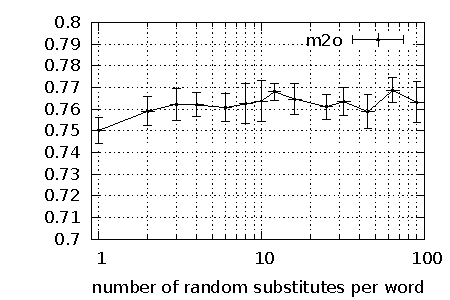
\includegraphics[width=0.5\linewidth]{plot-s.pdf}
%% 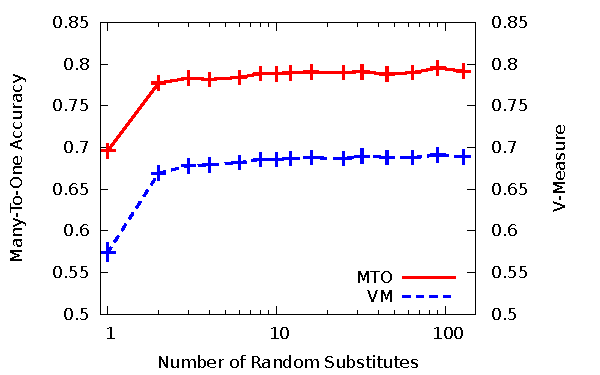
\includegraphics[width=.90\columnwidth]{plot-s-ins.pdf}
%% 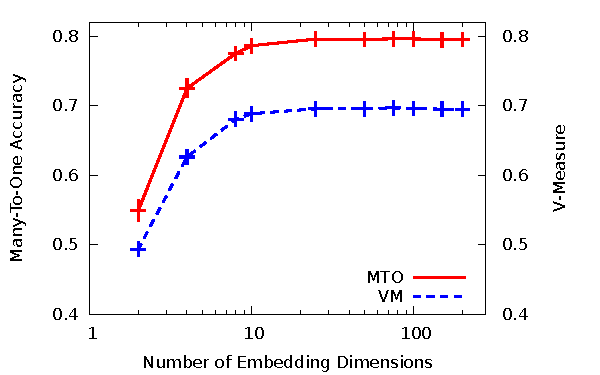
\includegraphics[width=0.90\columnwidth]{plot-d-ins.pdf}
%% 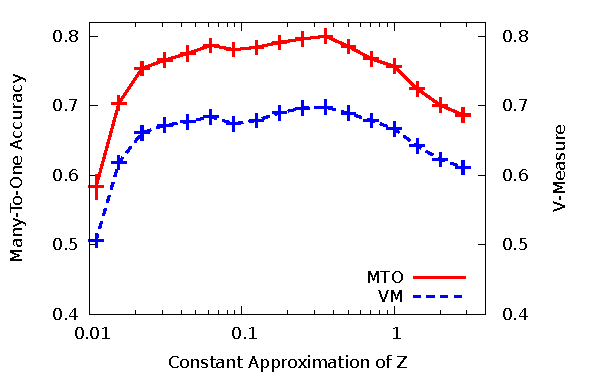
\includegraphics[width=0.90\columnwidth]{plot-z-ins.pdf}
%% %% \caption{\mto\ and \vm\ are not sensitive to the number of random substitutes
%% %% sampled per word instance.}
%% \caption{Sensitivity of instance-based POS induction performance on
%%   the PTB to (a) the number of sampled substitutes, (b) the number of
%%   embedding dimensions, (c) the constant approximation to the
%%   normalization constant $\tilde{Z}$.
%% }
%% \label{plot-s}
%% \end{figure}

%% % TODO: This goes to algorithm section:
%% %% S-CODE uses stochastic gradient ascent to find the $\phi_w, \psi_c$ embeddings
%% %% for words types and contextual features on a 25-dimensional unit sphere.  The algorithm
%% %% cycles through the word-features tuple data until it converges.  
%% We construct a vector representation for instances by concatenating the S-CODE
%% embedding of the target word $\phi_w$ with the average of sampled substitute
%% embeddings, $\overline{\psi_c}$.  The resulting $\phi_w \oplus
%% \overline{\psi_c}$ vectors are clustered using the k-means algorithm and the
%% cluster-id for each $\phi_w \oplus \overline{\psi_c}$ becomes the predicted
%% category of the corresponding word instance.  Using the default settings the
%% many-to-one accuracy on the PTB is \fwsxymto\ and the V-measure is \fwsxyvm.
%% %% Moved to appendix
%% %% To obtain a discrete representation of the context, the
%% %% random-substitutes algorithm pairs each word instance with a substitute
%% %% sampled from the pre-computed substitute vectors generated from the
%% %% word instance's context (see Section~\ref{sec:subcomp}) and word ($X$) --
%% %% random-substitute ($Y$) pairs are fed to the S-CODE as input.  It is
%% %% possible (and beneficial, see below) to run the random-substitutes
%% %% algorithm on the data more than once to generate more pairs from the
%% %% same substitute vectors. 
%% %% To obtain a discrete representation of the context, the
%% %% random--partitions algorithm first designates a random subset of
%% %% substitute vectors as centroids to partition the space, and then
%% %% associates each context with the partition defined by the closest
%% %% centroid in cosine distance.  Each partition thus defined gets a
%% %% unique id, and word ($X$) -- partition-id ($Y$) pairs are given to
%% %% S-CODE as input.  The algorithm uses stochastic gradient ascent to
%% %% find the $\phi_x, \psi_y$ embeddings for word and partition-id in
%% %% these pairs on a single 25-dimensional sphere.  The algorithm cycles
%% %% through the data until we get approximately 50 million updates.  The
%% %% resulting $\phi_x$ vectors are clustered using an instance weighted
%% %% k-means algorithm and the resulting groups are compared to the correct
%% %% part of speech tags.  Using default settings with 64K random
%% %% partitions the many-to-one accuracy is \rpmto\ and the V-measure is
%% %% \rpvm.
%% % \subsubsection*{Sensitivity Analysis}

%% To analyze the sensitivity of this result to our specific parameter
%% settings we ran a number of experiments where each parameter was
%% varied over a range of values.
%% %% \begin{figure}[ht] \centering
%% %% 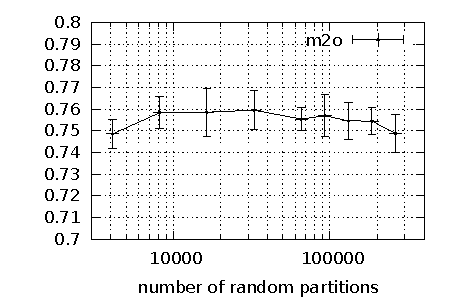
\includegraphics[width=0.5\linewidth]{plot-p.pdf}
%% %% \caption{\mto\ is not sensitive to the number of partitions used to
%% %%   discretize the substitute vector space within our experimental
%% %%   range.}
%% %% \label{plot-p}
%% %% \end{figure}
%% %% Figure~\ref{plot-p} gives results where the number of initial random
%% %% partitions is varied over a large range and shows the results to be
%% %% fairly stable across two orders of magnitude.

%% The first plot in Figure~\ref{plot-s} illustrates that the result is
%% fairly robust with respect to the number of random substitutes sampled
%% for each target word instance, as long as the training algorithm can
%% observe more than a few random substitutes per word.  The second plot
%% shows that at least 10 embedding dimensions are necessary to get
%% within 1\% of the best result, but there is no significant gain from
%% using more than 25 dimensions.  The third plot shows that the constant
%% $\tilde{Z}$ approximation can be varied within two orders of magnitude
%% without a significant performance drop in the scores.  For uniformly
%% distributed points on a 25 dimensional sphere, the expected $Z$ is
%% $0.146$.  In the experiments where we tested we found the real $Z$
%% always to be in the 0.140-0.170 range.  When the constant $\tilde{Z}$
%% estimate is too small, all points tend to converge to the same
%% location.  When $\tilde{Z}$ is too high, it prevents meaningful
%% clusters from coalescing.


%% \subsection{Morphological and Orthographic Features}
\label{sec:feat}

Clark \shortcite{Clark:2003:CDM:1067807.1067817} demonstrates that
using morphological and orthographic features significantly improves
part of speech induction with an HMM based model.
Section~\ref{sec:related} describes a number of other approaches that
show similar improvements.  We integrate additional features together
with substitutes by using the model described in Appendix~C.

%% In order to accommodate multiple feature types the CODE model in
%% Appendix~\ref{sec:codethr} needs to be extended to handle more than
%% two variables.  Globerson et al. \shortcite{globerson2007euclidean}
%% suggest the following likelihood function:

%% \begin{eqnarray}
%% &\ell(\phi,& \psi^{(1)}, \ldots, \psi^{(K)}) = \label{eq:multiscode}
%%   \sum_i^K w_i \sum_{x,y^{(i)}} \bar{p}(x,y^{(i)}) \log p(x,y^{(i)})
%% \end{eqnarray}

%% \noindent where $Y^{(1)}, \ldots, Y^{(K)}$ are $K$ different variables
%% whose empirical joint distributions with $X$,
%% $\bar{p}(x,y^{(1)})\ldots\bar{p}(x,y^{(K)})$, are known.
%% Eq.~\ref{eq:multiscode} then represents a set of CODE models
%% $p(x,y^{(k)})$ where each $Y^{(k)}$ has an embedding $\psi_y^{(k)}$
%% but all models share the same $\phi_x$ embedding.  The weights $w_k$
%% reflect the relative importance of each $Y^{(k)}$ and all embeddings
%% are mapped to unit-sphere.

%% We adopt this likelihood function, set all $w_k=1$, let $X$ represent
%% a word, $Y^{(1)}$ represent a random substitute, and $Y^{(2)}, \ldots,
%% Y^{(K)}$ stand for morphological and orthographic features of the word
%% thus each word is a (K+1)-tuple, $(X, Y^{(1)}, \hdots Y^{(K)})$.  With
%% this setup, the training procedure needs to change little: instead of
%% sampling a word -- random-substitute pair, the word --
%% random-substitute -- features tuple is sampled and input to the
%% gradient ascent algorithm.  The gradient search algorithm updates the
%% embeddings according to $p(x,y^{(i)})$ where $i=1\hdots k$ and no
%% updates are performed between $y^{(i)}$s since they do not have any
%% co-occurrence statistics and $x$ is the shared variable.

%% Word tuples might have null values due to the unobserved features.
%% For example, the word ``\textbf{car}'' has no morphological or
%% orthographic features therefore all the elements of the tuple have
%% null value except the word type ($X$) and the random-substitute
%% ($Y^{(1)}$).  We do not perform any pull or push updates on embeddings
%% during the gradient search if the corresponding $y^{(k)}$ is
%% null\footnote{$X$ and $Y^{(1)}$ represents the word type and
%%   random-substitute therefore they are always observed.}.

%% One problem with this setup is that unobserved features misguide the
%% gradient search algorithm and lead to a suboptimal convergence point.
%% For example, ``\textbf{car}'' and ``\textbf{red}'' belong to the
%% ``Noun'' and ``Adjective'' clusters, respectivly, and neither of them
%% have a morphological feature, thus their morphological features are
%% represented by a null value, ``X''.  However setting the unobserved
%% features of words from different clusters to ``X'' leads to a false
%% similarity between these words.  To solve this problem, 

The orthographic features we used are same with the ones in
\cite{yatbaz-sert-yuret:2012:EMNLP-CoNLL} with small modifications:
\begin{itemize}
\item Initial-Capital: this feature is generated for capitalized words
  with the exception of sentence initial words.
\item Number: this feature is generated when the instance starts with a
  digit.
\item Contains-Hyphen: this feature is generated for lowercase words
  with an internal hyphen.
\item Initial-Apostrophe: this feature is generated for instances that
  start with an apostrophe.
\end{itemize}

We generated morphological features using the unsupervised algorithm Morfessor
\cite{creutz05}.  Morfessor was trained on the WSJ section of the Penn Treebank
using default settings, and a perplexity threshold of 1\footnote{Let's put a
note on this}.  In our model, a word type consists of two parts: a stem and a
suffix part.  The suffix part is used as the morphological feature thus each
word type has only one morphological feature\footnote{We extracted the stem
  part by concatenating the splits until including the first ``STM'' labeled
split and the suffix part by concatenating rest of the splits.}.  The program
induced 5575 suffix types that are present in a total of 19223 word types.
Table~\ref{tab:sampleswithfeatures} presents the co-occurrence tuples of the
example sentence after incorporating the orthographic and morphological
features.
\begin{table*}[ht]
\centering
\footnotesize
\caption{The words of input sentence \textit{``Pierre Vinken, 61 years old, 
    will join the board as a nonexecutive director Nov.~29 .''} is represented 
  with their substitutes and features.  Words on the left 
  column presents the
  target word, words on the second column represents the context and
  instances on the rest of the columns are the features of the
  correponding target word.  Features without values are unobserved
  therefore set to null.}
\begin{tabular}{|lllllll|}
\hline
\textbf{Word} & {\bf Context} & {\bf Morphology} &
\specialcell{{\bf Initial}\\{\bf Capital}} & {\bf Number} &
\specialcell{{\bf Contains}\\{\bf Hypen}} &
\specialcell{{\bf Initial}\\{\bf Apostrophe}}
\\
\hline
W:Pierre & \textit{C:Mr.} & & {\it F:IC} &&&\\
W:Vinken & \textit{C:\unk} & & {\it F:IC} &&&\\
W:, & \textit{C:,} & & &&&\\
W:61 & \textit{C:48} & & & {\it F:N}&&\\
W:years & \textit{C:years} & {\it F:s} &&&&\\
W:old & \textit{C:old} & & &&&\\
W:join & \textit{C:head} &&&&&\\
W:the & \textit{C:its} &&&&&\\
W:board & \textit{C:company} &&&&&\\
W:as & \textit{C:as} &&&&&\\
W:a & \textit{C:a} &&&&&\\
W:nonexecutive & \textit{C:non-executive} &&&&&\\
W:director & \textit{C:chairman} & {\it F:or}&&&&\\
W:Nov. & \textit{C:May} &&{\it F:IC}&&&\\
W:29 & \textit{C:9} &&&{\it F:N}&&\\
W. & \textit{C:.} & &&&&\\
\hline
\end{tabular}
\label{tab:sampleswithfeatures}
\end{table*}

%% These suffixes were input to S-CODE as morphological features whenever
%% the associated word types were sampled.  In order to incorporate
%% morphological and orthographic features into
%% S-CODE we modified its input.  For each word -- random-substitute pair
%% generated as in the previous section, we added word -- feature pairs
%% to the input for each morphological and orthographic feature of the
%% word.  Words on average have 0.25 features associated with them.
%% This increased the number of pairs input to S-CODE from 14.1
%% million (12 substitutes per word) to 17.7 million (additional 0.25
%% features on average for each of the 14.1 million words).
Using the training settings of the previous section, the addition of
morphological and orthographic features increased the many-to-one score of the
random-substitute model to \fwsxymto\ and V-measure to \fwsxyvm.  Both these
results improve the state-of-the-art instance in part of speech induction
significantly as seen in Table~\ref{tab:results}.

%% \subsection{Summary}
%% \label{sec:expsum}

%% We presented methods to determine the best usage of substitute vectors
%% within the CODE framework and performed sensitivity analysis on the
%% model parameters to not only show the robustness but also to decide
%% the best configuration of S-CODE in modeling the co-occurrence of
%% words with their contexts.  To use the substitute vectors as
%% co-occurrences we discretized the substitute vectors using two
%% methods.  The first method (Section~\ref{sec:rpart}) selected 64K
%% random substitute vectors as the center of 64K partitions and then
%% assigned rest of the substitute vectors to the closest partition.  As
%% a result each word represented as a word -- partition-id pair which we
%% input to S-CODE. The second method (Section~\ref{sec:wordsub}) sampled
%% random substitutes from the substitute vectors using the fact that the
%% substitute vectors are probability distributions.  We fed the word --
%% random-substitute pairs into S-CODE.  Both methods significantly
%% outperform the syntagmatic bigram model (Section~\ref{sec:bigram}) on
%% the PTB.  Finally, Section~\ref{sec:feat} showed that adding
%% morphological and orthographic features improved the accuracy and we
%% achieved the state-of-the-art \mto\ and \vm\ accuracies on the PTB.

%% In the next section we extend our experiments to include more
%% languages to demonstrate the robustness of paradigmatic approach on
%% languages with different characteristics.

\subsection{Word vs. Instance-Based Induction}
\label{sec:typevsinstance}

Table~\ref{tab:results} shows that the overall many-to-one accuracy of
our instance based induction system is comparable to
\cite{yatbaz-sert-yuret:2012:EMNLP-CoNLL}\footnote{The difference is
  not statistically significant at $p=0.05$.} and significantly higher
than the other published results.  However Figure~\ref{fig:perplexity}
suggests that this summary hides the large difference in the answers
given by the different systems.  In this section we compare the
performance of our instance-based model to the word-based model of
\cite{yatbaz-sert-yuret:2012:EMNLP-CoNLL} on word types at different
levels of ambiguity.  We propose the gold-tag perplexity of a word as
a measure of its degree of ambiguity defined as follows:
\begin{equation*} \label{eq:tag-perp}
GP(w) = 2^{H(p_w)} = 2^{-\sum_{t} p_w(t)log_2 p_w(t)}
\end{equation*}
\noindent where $w$ is a word, $t$ is a tag, $p_w$ is the gold POS tag
distribution of the word $w$ and $H(p_w)$ is the entropy of the $p_w$
distribution.  A $GP$ of 1 for a word $w$ indicates that $w$ is always
associated with the same POS tag.  A word with $N$ equally probable
tags would have a $GP$ of $N$.

Figure~\ref{fig:perplexity} in the introduction plots the gold-tag
perplexity versus the smoothed \mto\ accuracy for the word-based and
the instance-based POS induction systems.  To compose the plot, we
found the best mapping from the induced clusters to the gold-standard
tags, then we computed the \mto\ accuracy for each word using this
mapping and plotted the \mto\ as a function of the word's $GP$.  We
used the Nadaraya-Watson kernel regression estimate
\cite{nadaraya1964estimating,watson1964smooth} with normal kernel of
bandwidth 1.0 to obtain smooth regression lines.  The figure shows
that the performance of the instance-based induction model does not
degrade as much as the word-based model as the ambiguity of the words
increase.  However, only 14.94\% of the instances in the PTB consists
of words with GP greater than 1.5 and 45.71\% consists of words with
GP exactly 1.  Thus, the overall accuracy numbers do not adequately
reflect the improvement on highly ambiguous words.

%% In the next section we apply the instance based model on 19 corpora in 15
%% different languages. 

%% Due to the one-tag-per-word nature of POS induction, the
%% type based model significantly outperforms the instance based one on the
%% unambiguous words.  Instance based model performs significantly better than the
%% type based model on the ambiguous words and assigns 1.34 tags per word.  
%% \subsection{Clustering Concatenation of Word and Context Embeddings (${\bf W}\oplus{\bf S}$)}
%% \label{sec:clustering-c}
%% Two models presented in earlier sections perform POS induction either
%% by assuming (Section~\ref{sec:clustering-w}) or discarding
%% (Section~\ref{sec:clustering-c}) the one-tag-per-word assumption.  In
%% this section we define a sparse-instance based model which clusters the
%% concatenation of ${\bf W}$ and ${\bf S}$ embeddings.  This model not
%% only tends to put instances of a word into the same cluster but
%% also performs instance based clustering by incorporating the word
%% and context information together.
%%
%% Similar to the previous models, we generate ${\bf W}$ -- ${\bf S}$
%% pairs as the input to S-CODE.  For each observed ${\bf W}$ -- ${\bf
%%   S}$ pair in the S-CODE input, corresponding 25-dimensional $\phi_w$
%% and $\psi_c$ embeddings are concatenated to create a 50-dimensional
%% representation.  We used the same experimental setting of the previous
%% section and predict the instance clusters according to the majority
%% cluster-id of the corresponding pairs.  The many-to-one accuracy of
%% this model is \wsxymto\ and the V-measure is \wsxyvm\ .
%% 
%% Table~\ref{tab:bins} presents the performance of the ${\bf
%%   W}\oplus{\bf S}$ based model over the subsets and it achieves
%% statistically better \mto\ than both of the ${\bf W}$ and ${\bf S}$
%% based models on ambiguous words.  Due to the bias towards to the
%% sparse clustering, sparse-instance based model statistically improves the
%% \mto\ accuracy on unambiguous words compared to the ${\bf S}$ based
%% model but it still can not achieve the performance of the ${\bf W}$
%% based model.  The ${\bf W}\oplus{\bf S}$ based model constructs instance 
%% based clusters that tend to assign instances of a word into the
%% same cluster which leads to a smaller average $GP$ than the ${\bf S}$
%% based model as shown in Table~\ref{tab:bins}.
%%
%% We don't really need this part
%% \subsubsection{Paradigmatic vs Syntagmatic Representations of Word Context}
%% \label{sec:bigram-instance}
%% In order to compare the instance clustering performance of the
%% paradigmatic and the syntagmatic context representations we use the
%% same 4 models defined in Section~\ref{sec:bigram-type}.  Following the
%% previous section we concatenate the 25-dimensional $\phi_x$ and
%% $\psi_y$ ($\psi_{y_{1}}$ and $\psi_{y_{2}}$ in the fourth model)
%% embeddings of the corresponding observed pairs (tuples in the fourth
%% model) and represent the first three models outputs with a
%% 50-dimensional vectors (75-dimensional vectors in the fourth model).
%% The resulting vectors are clustered using k-means algorithm with 128
%% restarts.
%% \begin{table}[ht]
%% \centering
%% \small
%% \caption{Accuracies of the instance based S-CODE models on the gold-tag
%%   perplexity separated subsets.}
%% \begin{tabular}{|l|l|l|l|}
%% \hline
%% Model & \specialcell{$GP < 1.75$\\$89\%$} & \specialcell{$GP \ge 1.75$\\$11\%$} & \specialcell{$GP \ge 1.0$\\$100\%$}\\
%% \hline
%% $X$ (word) - $Y$ (left bigram) & .5950 (.0051) & .4783 (.0005) & .5821 (.0041)\\
%% $X$ (word) - $Y$ (right bigram) & .6239 (.0049) & .3075 (.0153) & .5891 (.0046)\\
%% $X$ (word) - $Y$ (left and right bigram concatenation) & .7523 (.0065) & .4492 (.0240) & .7190 (.0049)\\
%% $X$ (word) - $Y_1$, $Y_2$ (left and right bigrams) & .6697 (.0065) & .4579 (.0052) & .6464 (.0051)\\
%% $X$ (word) - $Y$ (random substitutes) & .7322 (.0079) & .4671 (.0174) & .7030 (.0073)\\
%% \hline
%% \end{tabular}
%% \label{tab:instances}
%% \end{table}

%\subsection{Paradigmatic vs Syntagmatic Representations of Word Context}
\label{sec:pvss}

To get a direct comparison of the paradigmatic and syntagmatic context
representations we feed 4 different co-occurrences defined in
Section~\ref{sec:representation} into the S-CODE algorithm.  The first
model accepts word ($W$) - right bigram ($C$) pairs as the input, the
second model accepts word ($W$) - left bigram($C$) pairs as the input,
the third model accepts word ($W$) - concatenation of the left and
right bigrams ($C$) pairs \cite{mintz2003frequent} as the input and
the final model accepts words ($W$) - left bigram($C_1$) and right
bigram ($C_2$) tuples \cite{20674613} as the input to the S-CODE.
Finally, we cluster the word type embeddings ($W$) with k-means
algorithm and report the results on Table \ref{tab:syntagmatic}.
\begin{table*}[ht]
\centering
\caption{Summary of results in terms of the \mto\ and \vm\ scores of
  the S-CODE algorithm when the paradigmatic or syntagmatic
  representations are feed as an input.  Standard errors are given in
  parentheses when available.  Results of the statistically best
  performing system are written in bold.  We do not report the
  original results of Maron et al. \protect\shortcite{maron2010sphere}
  since our replication achieves higher accuracies.}
\begin{tabular}{|l|l|l|}
\hline
Input & \mto & \vm\\
\hline
$W$ (word) - $C$ (right bigram) & .6625 (.0115) & .5809 (.0066)\\
$W$ (word) - $C$ (left bigram) & .6604 (.0054) & .5983 (.0028)\\
$W$ (word) - $C$ (left and right bigram concatenation) & .7268 (.0091) & .6416 (.0052)\\
$W$ (word) - $C_1$, $C_2$ (left and right bigrams) & .7173 (.0061) & .6381 (.0032)\\
Maron et al. \shortcite{maron2010sphere}(replication)  & \bgmto & \bgvm \\
$W$ (word) - $C$ (random substitutes) & {\bf\wsmto} & {\bf\wsvm} \\
\hline
\end{tabular}
\label{tab:syntagmatic}
\end{table*}

To replicate the work of Maron et al. \shortcite{maron2010sphere} we
feed word ($W$) - right bigram ($C$) pairs as the input.  At the end
each word $w$ in the vocabulary ends up with two points on the sphere,
a $\phi_w$ point representing the behavior of $w$ as the left word of
a bigram and a $\psi_w$ point representing it as the right word.  The
two vectors for $w$ are concatenated to create a 50-dimensional
representation at the end.  These 50-dimensional vectors are clustered
using the k-means algorithm.  Maron et al. \shortcite{maron2010sphere}
report many-to-one scores of .6880 (.0016) for 45 clusters and .7150
(.0060) for 50 clusters (on the PTB).  Using our default settings the
bigram model achieves \bgmto\ \mto\ and \bgvm\ \vm\ accuracies.  Table
\ref{tab:syntagmatic} summarizes all the results and shows that the
paradigmatic representation accuracies are significantly higher than
the syntagmatic representation \mto\ and \vm\ accuracies.

\subsection{Multilingual Experiments}
\label{sec:multilang}
\noindent Following Christodoulopoulos et
al. \shortcite{christodoulopoulos-goldwater-steedman:2011:EMNLP}, we extend our
experiments to 8 languages from MULTEXT-East (Bulgarian, Czech, English,
Estonian, Hungarian, Romanian, Slovene and Serbian) \cite{citeulike:5820223}
and 10 languages from the CoNLL-X shared task (Bulgarian, Czech, Danish, Dutch,
German, Portuguese, Slovene, Spanish, Swedish and Turkish)
\cite{Buchholz:2006:CST:1596276.1596305}.  

To sample substitutes, we trained language models of Bulgarian, Czech,
Estonian, Romanian, Danish, German, Dutch, Portuguese, Spanish, Swedish and
Turkish with their corresponding TenTen corpora \cite{jakubivcek2013tenten},
and Hungarian, Slovene and Serbian with their corresponding Wikipedia dump
files\footnote{Latest Wikipedia dump files are freely available at
  \url{http://dumps.wikimedia.org/} and the text in the dump files can be
  extracted using WP2TXT (\url{http://wp2txt.rubyforge.org/})}.  Serbian shares
  a common basis with Crotian and Bosnian therefore we trained 3 different
  language models using Wikipedia dump files of Serbian together with these two
  languages and measured the perplexities on the MULTEXT-East Serbian corpus.
  We chose the Croatian language model since it achieved the lowest perplexity
  score and unknown word ratio on MULTEXT-East Serbian corpus.  We use ukWaC
  corpora to train English language models. 

We used the default settings in Section~\ref{sec:expset} and incorporated only
the orthographic features\footnote{All corpora (except German, Spanish and
Swedish) label the punctuation marks with the same gold-tag therefore we add an
extra {\em punctuation} feature for those languages.}.  Extracting
unsupervised morphological features for languages with different
characteristics would be of great value, but it is beyond the scope of this
paper.  For each language the number of induced clusters is set to the number
of tags in the gold-set.  To perform meaningful comparisons with the previous
work we train and evaluate our models on the training section of
MULTEXT-East\footnote{Languages of MULTEXT-East corpora do not tag the
punctuations, thus we add an extra tag for punctuations to the tag-set of these
languages.} and CONLL-X languages \cite{Lee:2010:STU:1870658.1870741}.

Table~\ref{tab:multiresults} presents the performance of our instance based
model on 19 corpora in 15 languages together with the corresponding best
published results from
$^\diamond$\protect\cite{yatbaz-sert-yuret:2012:EMNLP-CoNLL},
$^\ddagger$\protect\cite{blunsom-cohn:2011:ACL-HLT2011},
$^\star$\protect\cite{christodoulopoulos-goldwater-steedman:2011:EMNLP} and
$^\dagger$\protect\cite{Clark:2003:CDM:1067807.1067817}.  All of the
state-of-the-art systems in Table~\ref{tab:multiresults} are word-based and
incorporate morphological features. 
%%Multiple language section
\begin{table}[t]
\centering  \small
%% Table notation info
%% PYP is \ddagger
%% BMMM is \star
%% Clark is \dagger
%% kmeans is ^k
%% Yatbaz \diamond  
%% 
  \begin{tabular}{l|l|l|l|l|}
    \hline
    & Language   & Tags & \specialcell{Best\\ Published \\ \mto\ \ \vm\ } &
    \specialcell{Instance\\Based\\\mto\ / \vm\ }\\\hline 
    \multirow{1}{*}{\begin{sideways}\textbf{WSJ}\end{sideways}} 
    & English     & 45   & .802 / {\bf .721} $^\diamond$        &.795 / .691\\ 
    & & & &\\ \hline
    \multirow{8}{*}{\begin{sideways}\textbf{MULTEXT-East}\end{sideways}}
    & Bulgarian   & 12+1 & .665 / {\bf .556}$^\star$                  & .664 / .513\\ 
    & Czech       & 12+1 & .642 / {\bf.539}$^\star$                   & {\bf .705} / .511\\ 
    & English     & 12+1 & .733 / .633$^\star$                        & {\bf .835} / {\bf .661}\\ 
    & Estonian    & 11+1 & .644 / {\bf.533}$^\star$                   & .643 / .457\\ 
    & Hungarian   & 12+1 & {\bf .682} / {\bf.548}$^\star$             & .647/ .459\\
    & Romanian    & 14+1 & .611 / .523$^\star$                        & {\bf .660} / .528\\
    & Slovene     & 12+1 & {\bf .679} / {\bf.567}$^\star$             & .667 / .451\\
    & Serbian     & 12+1 & {\bf .641} / {\bf.510}$\dagger$            & .594/ .402\\
    \hline % Conll06 data
    \multirow{10}{*}{\begin{sideways}\textbf{CoNLL-X Shared Task}\end{sideways}}
    & Bulgarian   & 54   & .704 / {\bf.596}$\dagger$                  & {\bf .751} / .583\\
    & Czech       & 12   & .701$^\ddagger$ / .484$^\star$             & .701 / .486\\
    & Danish      & 25   & .761$^\ddagger$ / .591$^\star$             & .761 / .584\\
    & Dutch       & 13   & .711$^\ddagger$ / {\bf .547}$^\star$       & .712 / .537\\
    & German      & 54   & .744$^\star$ / {\bf .630}$\dagger$         & .749 / .618\\
    & Portuguese  & 22   & .785$^\ddagger$ / {\bf .639}$^\star$       & .782 / .607\\
    & Slovene     & 29   & .642$^\star$ / {\bf.539}$\dagger$          & .638 / .469\\
    & Spanish     & 47   & {\bf.788}$^\ddagger$ / {\bf .632}$^\star$  & .753/ .602\\
    & Swedish     & 41   & .682 / {\bf.589}$\dagger$                  & .681 / .546\\
    & Turkish     & 30   & .628 / .408$^\star$                        & .637 / .401\\ 
    \hline
  \end{tabular}
  \caption{The \mto\ and \vm\ scores on 19 corpora in 15 languages together
  with number of induced clusters.  Statistically significant results shown
  in bold ($p < 0.05$).
}  
  \label{tab:multiresults}
\end{table}


Our \mto\ results are lower than the best systems on all of data-sets that use
language models trained on the Wikipedia corpora.  ukWaC and TenTen corpora are
cleaner and tokenized better compared to the Wikipedia corpora.  These corpora
also have larger vocabulary sizes and lower out-of-vocabulary rates.  Thus
language models trained on these corpora have much lower perplexities and
generate better substitutes than the Wikipedia based models.  Our model has
lower \vm\ scores in spite of good \mto\ scores on 14 corpora which is
discussed in Section~\ref{sec:discuss}.

Among the languages for which clean language model corpora were available, our
model performs comparable to or significantly better than the best systems on
most languages.  We show significant improvements on MULTEXT-East Czech,
Romanian, and CoNLL-X Bulgarian.  Our model achieves the state-of-the-art \mto\
on MULTEXT-East English and scores comparable \mto\ with the best model on WSJ.
Our model shows comparable results on MULTEXT-East Bulgarian and Estonian, and
CoNLL-X Czech, Danish, Dutch, German, Portuguese, Swedish and Turkish in terms
of the \mto\ score.  One reason for comparably low \mto\ on Spanish might be
the absence of morphological features.

% TODO: describe the table.

%% Morphological features of each language are extracted by the
%% method described in Section~\ref{sec:feat}.  The details of the
%% language model training and feature extraction are detailed in
%% Appendix~D.
%% We ignore these results
%% %%Multiple language section
\begin{table*}[ht]
%% Table notation info
%% PYP is \ddagger
%% BMMM is \start
%% Clark is \dagger
%% kmeans is ^k
%% 
%  \small
  \centering
  \caption{The \mto\ and \vm\ scores of X+Y token clustering S-CODE on
    19 corpora in 15 languages together with the number of unique words and
    tags in gold--set which equals to number of induced clusters in
    all languages.  MULTEXT-East corpora do not tag the punctuation
    marks, thus we add an extra tag for punctuation and represent it
    with ``+1''.}
%  \begin{tabular}{|@{ }l@{ }|@{ }l@{ }|@{ }l@{ }|@{ }l@{ }|@{ }l@{ }|@{ }l@{ }|}
  \begin{tabular}{|l|l|l|l|l|l|}
        \hline
        & Language   & Types    & Tags & S-CODE X & S-CODE X+Y \\ \hline % Multext data
        \multirow{1}{*}{\begin{sideways}\textbf{WSJ}\end{sideways}} 
        & English    & 49,190  & 45 & .7667 / .6819 &.7030 / .6006\\
        & & & & &\\ \hline
        \multirow{8}{*}{\begin{sideways}\textbf{MULTEXT-East}\end{sideways}}
        & Bulgarian  & 16,352  & 12+1 & .6927 / .5341 & .6551 / .4644\\
        & Czech      & 19,115  & 12+1 & .7025 / .5020 & .6145 / .4031\\
        & English    & 9,773   & 12+1 & .8239 / .6631 & .7697 / .5977\\
        & Estonian   & 17,845  & 11+1 & .6612 / .4469 & .5934 / .3509\\
        & Hungarian  & 20,321  & 12+1 & .6900 / .4972 & .6235 / .4152\\
        & Romanian   & 15,189  & 14+1 & .6412 / .5004 & .5931 / .4185\\
        & Slovene    & 17,871  & 12+1 & .6914 / .4951 & .6466 / .4119\\
        & Serbian    & 18,095  & 12+1 & .6244 / .4473 & .5622 / .3466\\
        \hline % Conll06 data
        \multirow{10}{*}{\begin{sideways}\textbf{CoNLL-X Shared Task}\end{sideways}}
        & Bulgarian  & 32,439  & 54 & .7328 / .5781 & .6615 / .4821\\
        & Czech      & 130,208 & 12 & .6739 / .4838 & .6082 / .3566\\
        & Danish     & 18,356  & 25 & .7236 / .5583 & .6210 / .4351\\
        & Dutch      & 28,393  & 13 & .6957 / .5331 & .6168 / .4000\\
        & German     & 72,326  & 54 & .7669 / .6308 & .6484 / .5083\\
        & Portuguese & 28,931  & 22 & .7479 / .5798 & .6734 / .4859\\
        & Slovene    & 7,128   & 29 & .6513 / .4957 & .5918 / .4164\\
        & Spanish    & 16,458  & 47 & .7479 / .6086 & .6739 / .5142\\
        & Swedish    & 20,057  & 41 & .6962 / .5674 & .5779 / .4385\\
        & Turkish    & 17,563  & 30 & .6239 / .3823 & .5910 / .3309\\ \hline
    \end{tabular}
  \label{tab:multiresults}
\end{table*}

%% \subsubsection{Results}
%% \label{sec:multires}
%% For each language we report results of three models that cluster: (1)
%% word embeddings ({\em CLU-W}), (2) word embeddings with orthographic
%% features ({\em CLU-W+O}) and (3) word embeddings with both orthographic
%% and morphological features ({\em CLU-W+O+M}).  
%% As a baseline model we chose the syntagmatic bigram version of S-CODE
%% described in Section~\ref{sec:pvss} which is a very strong baseline
%% compared to the ones used in
%% \cite{christodoulopoulos-goldwater-steedman:2011:EMNLP}.
%% Table~\ref{tab:multiresults} summarizes the \mto\ and \vm\ scores of
%% our models together with the syntagmatic bigram baseline and the best
%% published accuracies on each language corpus.
%% {\em CLU-W} significantly outperforms the syntagmatic bigram baseline
%% in both \mto\ and \vm\ scores on 14 languages.  {\em CLU-W+O+M} has
%% the state-of-the-art \mto\ and \vm\ accuracy on the PTB.  {\em
%%   CLU-W+O} and {\em CLU-W+O+M} achieve the highest \mto\ scores on all
%% languages of MULTEXT-East corpora while scoring the highest \vm\
%% accuracies on English and Romanian.  On the CoNLL-X languages our
%% models perform better than the best published \mto\ or \vm\ accuracies
%% on 10 languages.


\section{Discussion}
\label{sec:discuss}

In this section we perform further analysis on the clustering output of our
model.  The example below illustrates the advantage of the
instance-based approach:

%% \begin{figure}[ht]
%%   %  \begin{minipage}[c]{\columnwidth}
     \begin{tabular}{ll}
      (1) & $\hdots$ it will also {\bf offer} buyers the option $\hdots$\\
      &{\bf Substitutes:} give, help, attract\\ 
      (2) & The {\bf offer} is being launched $\hdots$\\ 
      &{\bf Substitutes:} campaign, project, scheme\\ 
    \end{tabular}
 %%   \caption{Ambiguous occurrences of the word {\em offer}.}
 %%   \label{fig:typelimitation}
 %%   %\end{minipage} \hfill
 %% \end{figure}

The word {\bf offer} is a {\em verb} in the first sentence and a {\em
  noun} in the second one.  Clustering the word embeddings can not
distinguish the different occurrences of the words
\cite{yatbaz-sert-yuret:2012:EMNLP-CoNLL}.  On the other hand, the
substitutes of {\em offer} in the two sentences can disambiguate the
correct category of the corresponding occurrences.  In our actual
experiments our instance based representation distinguishes the
instances of {\bf offer} as {\em noun} (cluster 26 and 12) and {\em
  verb} (cluster 35).

To illustrate how words are distributed in the induced clusters, we
compare the most frequent clusters of our model in Section~\ref{sec:instance}
with the most frequent gold-tags of PTB in Figure~\ref{plot-hinton}.  
%%We also discuss the effect of coarse gold-tag sets
%%on our model performance.
\begin{figure}[h] \centering
%\vspace*{-10mm}
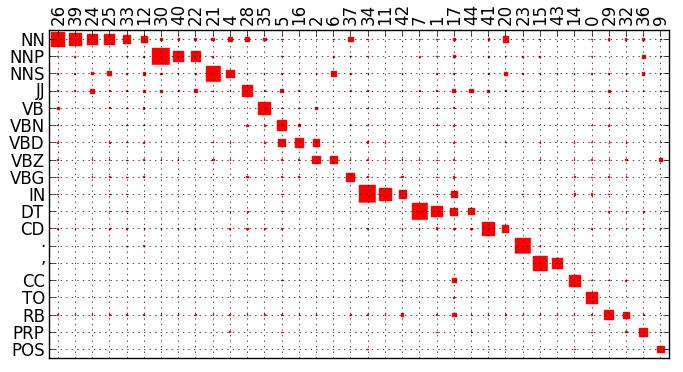
\includegraphics[width=1\columnwidth]{hinton.png}
\caption{Each row corresponds to a gold tag and each column is an
  induced tag in the Hinton diagram above.  The area of each square is
  proportional to the joint probability of the given tag and cluster.
}
  \label{plot-hinton}
\end{figure}

%% Figure~\ref{plot-hinton} is the Hinton diagram of the PTB showing the
%% relationship between gold tags and clusters\footnote{For simplicity only the
%% most frequent gold-tags and clusters are presented.} from the experiment in
%% Section~\ref{sec:instance}. 
The low \vm\ performance of our instance-based model compared to the
state-of-the-art word-based systems on some languages is due to the
completeness part of the \vm\ score.  The Hinton diagram in
Figure~\ref{plot-hinton} shows that large gold-tag groups are split
into several clusters based on the substitutability of words in that
particular cluster (rows of the Hinton diagram).  For example, proper
nouns ({\em NNP}) are split into three major clusters such that titles
like {\em Mr.} or person names are in (40), nationality or country
related words like {\em Japanese} or {U.S} are in (22), and the rest
of the proper nouns in cluster (30).

The gold-tags of PTB, on the other hand, do not always respect whether
words with the same tag are substitutable for one another.
Freudenthal et al.  \shortcite{freudenthal2005resolution} argues, from
the child language acquisition perspective, that the standard
linguistic definition of syntactic groups requires the
substitutability of words in a syntactic category.  Word pairs that
are placed in the same category in the PTB, such as ``Mr.'' and
``Friday'', ``be'' and ``run'', ``not'' and ``gladly'', ``of'' and
``into'' are clearly not generally substitutable.

Another noteworty example of completeness error is that our model splits the
punctuation mark ({\em ,}) class of PTB into the clusters 15 and 43 based on
the different usage patterns.  The majority of the ({\em ,}) instances in
cluster 15 are used in relative clauses, reported speech clauses or
conjunctions while cluster 43 generally consists of ({\em ,}) instances that
are used in non-essential clauses (ex: Time, the largest newsweekly, \ldots). 

%% Another source of completeness error in our model is the split of word
%% instances into several clusters.  For example, all instances of the
%% punctuation mark ({\em ,}) are tagged with same gold-tag in PTB,
%% however our model splits them into cluster 15 and 43 based on usage.

%% To decide whether the completeness or substitutability are better
%% measurement of POS induction, one can perform extrinsic evaluation
%% like parsing or machine translation.

%% Whether gold standard part of speech tags or distributional categories are
%% better suited to applications like parsing or machine translation can be best
%% decided using extrinsic evaluation.  In this study we evaluate our results by
%% comparing them to gold standard part of speech tags and leave the extrinsic
%% evaluations of the induced tags for future work.
%% Here are the some examples from clusters of our model:
%% \begin{itemize}
%%   \item Proper nouns ({\em NNP}) are split into three major clusters such that
%%   titles like {\em Mr.} and person names are in (40), nationality, country or
%%   time related words like {\em Japanese, U.S or Friday} are in (22), and the
%%   rest of the proper nouns in cluster (30).
%% \item Auxiliary verbs (10) and the verb ``say'' (22) have been split
%%   from the general verb clusters (12) and (7).
%% \item Determiners ``the'' (40), ``a'' (15), and capitalized
%%   ``The'', ``A'' (6) have been split into their own clusters.
%% \item Prepositions ``of'' (19), and ``by'', ``at'' (17) have been
%%   split from the general preposition cluster (8).
%% \end{itemize}
%% Nevertheless there are some homogeneity errors as well:
%% \begin{itemize} 
%% \item The adjective cluster (5) also has some noun members probably
%%   due to the difficulty of separating noun-noun compounds from
%%   adjective modification.
%% \item Cluster (6) contains capitalized words that span a number of
%%   categories.
%% \end{itemize}
%% A comparison of morphological structures might be helpful.
%% 
%% Most closed-class items are cleanly separated into their own clusters
%% as seen in the lower right hand corner of the diagram. 
% The sentences in Figure~\ref{fig:typelimitation} illustrates the limitation
% of clustering word embeddings.  

%% The completeness errors become more noticeable on languages with
%% coarse tag-sets thus our models perform worse than the best published
%% models on 6 of MULTEXT-East languages in terms of \vm\ scores while
%% achieving the state-of-the-art \mto\ scores on the same languages as
%% shown on Table~\ref{tab:multiresults}.  On CONLL-X languages the
%% effect of completeness errors is less noticeable since all languages
%% except Czech and Dutch have fine grained tag-sets.

%% The completeness errors are not surprising given that the words that
%% have been split are not generally substitutable with the other members
%% of their gold-tag set category.  Thus it can be argued that metrics
%% that emphasize homogeneity such as \mto\ are more appropriate in this
%% context than metrics that average homogeneity and completeness such as
%% \vm\ as long as the number of clusters is controlled.

%  There are two concerns inherent in all distributional methods: (i)
%  words that are generally substitutable like ``the'' and ``its'' are
%  placed in separate categories ({\sc dt} and {\sc prp\$}) by the gold
%  standard, (ii) words that are generally not substitutable like ``do''
%  and ``put'' are placed in the same category ({\sc vb}).  Freudenthal
%  et al. \shortcite{freudenthal2005resolution} point out that categories
%  with unsubstitutable words fail the standard linguistic definition of
%  a syntactic category and children do not seem to make errors of
%  substituting such words in utterances (e.g. {\em``What do you want?''}
%  vs. {\em *``What put you want?''}).  Whether gold standard part of
%  speech tags or distributional categories are better suited to
%  applications like parsing or machine translation can be best decided
%  using extrinsic evaluation.  In this study we evaluate our results by
%  comparing them to gold standard part of speech tags and leave the
%  extrinsic evaluation of the induced tags for future work.

%\subsection{Representing Word Context}
\label{sec:representation}

% example substitute vectors (both syntactic and semantic)

In this section we demonstrate the different contextual representations in the
part-of-speech induction (aka. syntactic word categorization) literature and
introduce the substitute words as an alternative to the current context
representations.  In the rest of the paper the words in the vocabulary are
referred as {\em types} and the instances of types are referred as {\em
instances}.

The contextual representations can be categorized into three groups
based on the way they incorporate the local context information of the
target type or instance: (1) syntagmatic representation, (2) Hidden
Markov Models (HMM) and (3) paradigmatic representation.  These
representations can be further subdivided into two subgroups based on
whether they group the types or the instances.

%\subsection{Co-occurrences}
\paragraph{Syntagmatic Representation}

In syntagmatic representation the context is defined with the
neighboring words, typically co-occurrences with a single word on the
left or a single word on the right word called a ``frame'' (e.g., {\em
  {\bf the} dog {\bf is}; {\bf the} cat {\bf is}})
\cite{SchutzePe93,redington1998distributional,mintz2003frequent,20674613,lamar-EtAl:2010:Short,maron2010sphere}.
Turney and Pantel \shortcite{DBLP:journals/jair/TurneyP10} give a
broad overview of syntagmatic approaches and their applications within
the Vector Space Modeling framework.  Depending on the way they
incorporate co-occurences, these models can perform hard (type based)
or soft (instance based) clustering.

Sch\"{u}tze \shortcite{SchutzePe93} represented the context of a word
type by concatenating its left and right co-occurrence vectors.  These
vectors were calculated for each type by using the left and the right
neighbors of the type instances therefore they characterize the
distribution of the left and right neighboring instances of the type.
One constraint of this representation is that it represents types
rather than instances thus it is not possible to group the instances of
any type into the separate categories.

Mintz \shortcite{mintz2003frequent} showed on a subset of child
directed speech corpus (CHILDES) \cite{macwhinney2000childes} that
non-adjacent high frequent bigram frames are useful for the language
learners on the syntactic categorization of the intances.  For example,
the intances that are observed at ``\_'' in the frame ``{\em {\bf the}
  \_ {\bf is}}'' are assigned to the same category.  Using the top-45
frequent frames Mintz achieved an average of 98\% unsupervised
accuracy\footnote{Unsupervised accuracy was defined as the number of
  hits (when two intervening instances that observed in the frame are
  from the same category) divided by number of false alarms (when two
  intervening instances that observed in the frame are from different
  categories).}.  The main limitation of the top-45 frequent frames is
that they could only analyze the 6\% of the instances on average due to
the sparsity.  Another drawback is that the instances with only one
common neighbors could not exchange information.

St Clair et al.  \shortcite{20674613} extended the work of Mintz
\shortcite{mintz2003frequent} and introduced the flexible bigram
frames which represent the context by using the left and the right
bigrams separately.  As a result instances with a common left or right
bigram can exchange information and might be grouped together.  For
instance, two instances that are observed at ```\_'' in ``{\em {\bf the}
  \_ {\bf is}}'' and ``{\em {\bf a} \_ {\bf is}}'' can be categorized
together due to the shared right bigram ``{\em{\bf is}}''.  Using a
feed forward connectionist model they showed that the flexible frames
are statistically better than the frequent frames in terms of the
supervised accuracy\footnote{In order to perform meaningful
  comparisons they used all of the frequent frames instead of the
  top-45 ones.}.  They also showed that representing instance contexts
only with the left or the right bigram is statistically better than
the frequent frames but worse than the flexible frames in terms of
supervised accuracy.  Both Mintz \shortcite{mintz2003frequent} and St
Clair \shortcite{20674613} did not report any results with contexts
larger than bigram since as the context is enriched, the re-occurrence
frequency of a frame becomes lower which causes the data sparsity
\cite{manning99foundations}.

%\subsection{HMM}
\paragraph{HMM} 
Prototypical HMM uses a bigram structure where instances are generated by
latent categories and learns the latent category sequence that
generates the given word sequence instead of clustering instances
directly
\cite{Brown:1992:CNG:176313.176316,blunsom-cohn:2011:ACL-HLT2011,goldwater-griffiths:2007:ACLMain,johnson:2007:EMNLP-CoNLL2007,Ganchev:2010:PRS:1859890.1859918,bergkirkpatrick-klein:2010:ACL,Lee:2010:STU:1870658.1870741}.
The POS induction literature focused on the first and second order
HMMs since the higher order HMMs have additional complicating
factors\footnote{The number of parameters in a prototypical HMM
  quadratically increases as the HMM order increases.}  and require
more complex training procedures \cite{johnson:2007:EMNLP-CoNLL2007}.
Depending on the design and the training procedure HMM models can
group types or instances which are detailed in Section \ref{sec:related}.

%\subsection{Substitute words}
\paragraph{Paradigmatic Representation} 

In the paradigmatic representation context is defined as the distribution of
the substitute words in that context.  Sch\"{u}tze
\shortcite{Schutze:1995:DPT:976973.976994} incorporates paradigmatic
information by concatenating the left co-occurrence and the right co-occurrence
vectors of the right and the left intances, respectively and grouped the instances
that have similar vectors.  The vectors from the neighbors include potential
substitutes.  Yatbaz et al. \shortcite{yatbaz-sert-yuret:2012:EMNLP-CoNLL}
calculate the most likely substitute words of a word in a given context and
clusters the types that have similar substitutes.

Our paradigmatic representation is related to substitute distributions used in
\cite{yatbaz-sert-yuret:2012:EMNLP-CoNLL}.  This method improves on their
foundation from two aspects: (1) it can cluster instances and (2) it models each
features separately.  Moreover we apply our model on 19 corpora in 15
languages. 

Similarly, Sch{\"u}tze and Pedersen \shortcite{SchutzePe93} define the
words that frequently co-occur together as the {\em syntagmatic
  associates} and words that have similar left and right neighbors as
the {\em paradigmatic parallels}.  We find that representing the
paradigmatic axis more directly using substitute vectors rather than
frequent neighbors improves part of speech induction.

Sahlgren \shortcite{sahlgren2006word} gives a detailed analysis of
paradigmatic and syntagmatic relations in the context of word-space
models used to represent the word meanings.  Sahlgren's paradigmatic
model represents word types using co-occurrence counts of their
frequent neighbors, in contrast to his syntagmatic model that
represents word types using counts of contexts (documents, sentences)
they occur in.  Our substitute vectors do not represent word types at
all, but {\em contexts of word instances} using probabilities of likely
substitutes.  Sahlgren finds that in word-spaces built by frequent
neighbor vectors, more nearest neighbors share the same part of speech
compared to word-spaces built by context vectors.



\section{Contributions}
\label{sec:contrib}
Our main contributions can be summarized as follows:
\begin{itemize}
\item We introduced an instance based POS induction system that can
  handle ambiguous words and is competitive with the word-based systems in
  overall accuracy.  
\item We extended the S-CODE framework to handle more than two categorical
  variables. 
\item Our instance based system scores 79.5\% many-to-one accuracy on
  the Penn Treebank and achieves results that are significantly better
  than or comparable with the best published systems on 12 out of 19
  corpora in 15 languages.
\item All our code and data, including the substitute vectors for the
  PTB, MULTEXT-East and CoNLL-X shared task corpora are available
  at the authors' website at \mbox{\url{xxx.xxx.xxx}}.
\end{itemize}


\section*{Acknowledgements}
We would like to thank Adam Kilgarriff and the Sketch
Engine\footnote{\url{https://www.sketchengine.co.uk}} team for making
their corpora available to us.  This work was supported in part by the
Scientific and Technical Research Council of Turkey (T\"{U}B\.{I}TAK
Project 112E277).

%%% \section{Co-occurrence Modeling}
%% \label{sec:code}

\appendix
%% %%\appendixsection{Algorithm}
%% %%\label{sec:algorithm}
%% %% [!! remove this part]
%% %% In this section, we briefly describe the components of our algorithm.
%% %% Section~\ref{sec:subcomp} presents the motive and the method for
%% %% computation of substitute vectors, our paradigmatic representations
%% %% for the word contexts.  We combine the substitute vectors with the
%% %% identity and features of the target word for part of speech induction
%% %% using the a co-occurrence modeling framework.
%% 
%% \appendixsection{Computation of Substitute Distributions}
%% \label{app:subcomp}
%% 
%% In this study, we predict the syntactic category of a word in a given
%% context based on its substitute distribution.  The sample space of the
%% substitute distribution is the vocabulary of the language model
%% including the unknown word tag \unk.  Note that the substitute
%% distribution is a function of the context only and is indifferent to
%% the target word.
%% 
%% %% The dimensions of the
%% %% substitute distribution represent words in the vocabulary of the
%% %% language model, and the entries in the substitute distribution
%% %% represent the probability of those words being used in the given
%% %% context.  
%% 
%% % how are the substitutes computed
%% It is best to use both the left and the right context when estimating
%% the probabilities for potential lexical substitutes.  For example, in
%% \emph{``He lived in San Francisco suburbs.''}, the instance \emph{San}
%% would be difficult to guess from the left context but it is almost
%% certain looking at the right context.  We define $c_w$ as the $2n-1$
%% word window centered around the target word position: $w_{-n+1} \ldots
%% w_0 \ldots w_{n-1}$ ($n=4$ is the n-gram order we have used).  The
%% probability of a substitute word $w$ in a given context $c_w$ can be
%% estimated as:
%% \begin{eqnarray}
%%   \label{eq:lm1}P(w_0 = w | c_w) & \propto & P(w_{-n+1}\ldots w_0\ldots w_{n-1})\\
%%   \label{eq:lm2}& = & P(w_{-n+1})P(w_{-n+2}|w_{-n+1})\nonumber\\
%%   &&\ldots P(w_{n-1}|w_{-n+1}^{n-2})\\
%%   \label{eq:lm3}& \approx & P(w_0| w_{-n+1}^{-1})P(w_{1}|w_{-n+2}^0)\nonumber\\
%%   &&\ldots P(w_{n-1}|w_0^{n-2})
%% \end{eqnarray}
%% where $w_i^j$ represents the sequence of words $w_i w_{i+1} \ldots
%% w_{j}$.  In Equation \ref{eq:lm1}, $P(w|c_w)$ is proportional to
%% $P(w_{-n+1}\ldots w_0 \ldots w_{n-1})$ because the words of the
%% context are fixed.  Terms without $w_0$ are identical for each
%% substitute in Equation \ref{eq:lm2} therefore they have been dropped
%% in Equation \ref{eq:lm3}.  Finally, because of the Markov property of
%% n-gram language model, only the closest $n-1$ words are used in the
%% experiments.
%% 
%% Near the sentence boundaries the appropriate terms were truncated in
%% Equation \ref{eq:lm3}.  Specifically, at the beginning of the sentence
%% shorter n-gram contexts were used and at the end of the sentence terms
%% beyond the end-of-sentence instance were dropped.
%% 
%% To obtain a discrete representation of the context, the
%% random-substitutes algorithm pairs each word instance with a substitute
%% sampled from the pre-computed substitute distribution generated from
%% the word instance's context and then word ($W$) -- random-substitute
%% ($S$) pairs are fed to the S-CODE algotihm as input.
%% 
%% \appendixsection{The CODE and S-CODE Models}
%%  \label{app:codethr}
%%  {\bf This section will be remoded after Dyuret's tuple sampling comments}
%% In this section we review the unsupervised method that we use to model
%% co-occurrence statistics: the Co-occurrence Data Embedding (CODE)\
%% \cite{globerson2007euclidean} method and its spherical extension (S-CODE)
%% introduced by \cite{maron2010sphere}.
%% 
%% Let $W$ and $C$ be two categorical variables with finite cardinalities
%% $|W|$ and $|C|$.  We observe a set of pairs $\{w_i, c_i\}_{i=1}^n$
%% drawn IID from the joint distribution of $W$ and $C$.  The basic idea
%% behind CODE and related methods is to represent (embed) each value of
%% $W$ and each value of $C$ as points in a common Euclidean space
%% $\mathbf{R}^d$ such that values that frequently co-occur lie close to
%% each other.  There are several ways to formalize the relationship
%% between the distances and co-occurrence statistics, in this paper we
%% use the following:
%% \begin{equation} \label{eq:probability}
%% p(w,c) = \frac{1}{Z} \bar{p}(w) \bar{p}(c) e^{-d^2_{w,c}}
%% \end{equation}
%% \noindent where $d^2_{w,c}$ is the squared distance between the
%% embeddings of $w$ and $c$, $\bar{p}(w)$ and $\bar{p}(c)$ are empirical
%% probabilities, and $Z=\sum_{w,c} \bar{p}(w) \bar{p}(c) e^{-d^2_{w,c}}$
%% is a normalization term.  If we use the notation $\phi_w$ for the
%% point corresponding to $w$ and $\psi_c$ for the point corresponding to
%% $c$ then $d^2_{w,c} = \|\phi_w-\psi_c\|^2$.  The log-likelihood of a
%% given embedding $\ell(\phi, \psi)$ can be expressed as:
%% \begin{eqnarray}
%% &&\ell(\phi, \psi) = \sum_{w,c} \bar{p}(w,c) \log p(w,c) \label{eq:likelihood} \\
%% &&= \sum_{w,c} \bar{p}(w,c) (-\log Z + \log \bar{p}(w)\bar{p}(c) - d^2_{w,c}) \nonumber \\
%% &&= -\log Z + \mathit{const} - \sum_{w,c} \bar{p}(w,c) d^2_{w,c} \nonumber
%% \end{eqnarray}
%% The likelihood is not convex in $\phi$ and $\psi$.  We use gradient
%% ascent to find an approximate solution for a set of $\phi_w$, $\psi_c$
%% that maximize the likelihood.  The gradient of the $d^2_{w,c}$ term
%% pulls neighbors closer in proportion to the empirical joint
%% probability:
%% \begin{equation}
%% \frac{\partial}{\partial\phi_w} \sum_{w,c} -\bar{p}(w,c) d^2_{w,c} =
%% \sum_y 2 \bar{p}(w,c) (\psi_c - \phi_w) \label{eq:attract}
%% \end{equation}
%% The gradient of the $Z$ term pushes neighbors apart in proportion to the
%% estimated joint probability:
%% \begin{equation}
%% \frac{\partial}{\partial\phi_x} (-\log Z) = \sum_y 2 p(w,c) (\phi_w -
%% \psi_c) \label{eq:repulse}
%% \end{equation}
%% Thus the net effect is to pull pairs together if their estimated
%% probability is less than the empirical probability and to push them
%% apart otherwise.  The gradients with respect to $\psi_c$ are similar.
%% S-CODE \cite{maron2010sphere} additionally restricts all $\phi_w$ and
%% $\psi_c$ to lie on the unit sphere.  With this restriction, $Z$ stays
%% around a fixed value during gradient ascent.  This allows S-CODE to
%% substitute an approximate constant $\tilde{Z}$ in gradient
%% calculations for the real $Z$ for computational efficiency.  In our
%% experiments, we used S-CODE with its sampling based stochastic
%% gradient ascent algorithm and smoothly decreasing learning rate.
%%  
\appendixsection{S-CODE with More than Two Variables}
\label{app:multiscode}
In this section we modify the S-CODE model to handle more than two variables. 
Let $W$ and $F^{(i)}$, where $i=1\ldots K$, be $K+1$ categorical
variables with finite cardinalities $|W|$ and $|F^{(i)}|$.  We observe a set of
tuples $\{w_j, f^{(1)}_j, \hdots, f^{(K)}_j\}_{j=1}^n$ drawn IID from the joint
distribution $\bar{p}(w, f^{(1)}, \hdots, f^{(K)})$, respectively.
Globerson et.  al \shortcite{globerson2007euclidean} suggest the following
likelihood function:

\begin{table}[ht]
  \footnotesize
  \begin{eqnarray}
    \ell(\phi, \psi^{(1)}, \ldots, \psi^{(K)}) =  \label{eq:multicode}
    \sum_{i=1}^K \sum_{w,f^{(i)}} \bar{p}(w,f^{(i)}) \log p(w,f^{(i)})
  \end{eqnarray}
\end{table}
\noindent where $\bar{p}(w, f^{(i)})$ is the empirical joint distribution of
$W$ with feature $F^{(i)}$ whose empirical joint distribution is known.  The
likelihood then represents a set of S-CODE models $p(w,f^{(i)})$ where each
$F^{(i)}$ has an embedding $\psi_f^{(i)}$ and all models share the same
$\phi_w$ embedding.

With this setup, the training procedure needs to change little: instead of
sampling a word ($w$) -- context ($c$), the word ($w$) -- feature $f^{(1)}$ --
$\hdots$ -- $f^{(K)}$ tuple is sampled and input to the gradient ascent
algorithm.  The gradient search algorithm updates the embeddings according to
$p(w,f^{(i)})$ and no updates are performed between any features since $w$ is
the only shared variable.

Tuples might have null values due to unobserved features.  For example in the
case of POS induction, the word ``\textbf{car}'' has no morphological or
orthographic features therefore all the elements of the tuple have null value
except the word type ($w$) and the contextual feature ($f_1$).  We do not
perform any pull or push updates on embeddings during the gradient search if
the corresponding $f^{(i)}$ is null.  In our setup $w$ and $f_1$ represents the
word type and contextual feature therefore they are always observed.

%% \appendixsection{Language Statistics}
%% \label{app:language}
%% This section explains the language model training and feature
%% extraction of each language that we apply our model in
%% Section~\ref{sec:multilang}.  

%% \paragraph{Statictical Language Modeling}For all languages except
%% Serbian, English and Turkish, we train the language models by using
%% the corresponding Wikipedia dump files\footnote{Latest Wikipedia dump
%%   files are freely available at \url{http://dumps.wikimedia.org/} and
%%   the text in the dump files can be extracted using WP2TXT
%%   (\url{http://wp2txt.rubyforge.org/})}.  Serbian shares a common
%% basis with Croatian and Bosnian therefore we trained 3 different
%% language models using Wikipedia dump files of Serbian together with
%% these two languages and measured the perplexities on the MULTEXT-East
%% Serbian corpus.  We chose the Croatian language model since it
%% achieved the lowest perplexity score and unknown word ratio on the
%% MULTEXT-East Serbian corpus.  To train the statistical language model
%% of English, we use Wall Street Journal data (1987-1994) extracted from
%% CSR-III Text \cite{csr3text} (excluding sections of the PTB) and for
%% the Turkish language modeling we use the web corpus collected from
%% Turkish news and blog sites \cite{sak2008turkish}.  
%% 
%% In order to reduce the unknown word ratio of resource poor languages
%% and to standardize the process we set the vocabulary threshold to 2
%% for all languages except English.  English has a relatively low
%% unknown word ratio therefore we set the threshold to 20 instead of 2.
%% Table~\ref{tab:lmstatistics} summarizes the language model related
%% statistics and scores that vary across the languages in terms of
%% quality and quantity.

%% \paragraph{Feature extraction}Morphological features of each language
%% are extracted using the training sections of the corresponding
%% MULTEXT-East and CoNLL-X corpora.  We don't use the language model
%% corpora to extract morphological features.  Number of morphological
%% feature of each language is presented in Table~\ref{tab:lmstatistics}.
%% We use the same set of orthographic features described in
%% Section~\ref{sec:feat} except we add an ``Only-Punctuation'' feature
%% to the languages of MULTEXT-East corpora.  The ``Only-Punctuation''
%% feature is generated when a instance only consists of punctuation
%% characters.
%% 
%% \begin{table*}[ht]
%  \small
  \centering
  \caption{Last two columns
    present the number of induced suffix parts and word types with
    these suffix parts after the morphological feature extraction.}
  \begin{tabular}{@{ }l@{ }|@{ }l@{ }|@{ }c@{ }|@{ }c@{ }|c@{ }|@{ }c@{ }|@{ }c@{ }|@{ }c@{ }|@{ }c@{ }|}
    \hline
    & & \multicolumn{2}{@{ }c@{ }|}{Language Model} & \multicolumn{5}{@{ }c@{ }|}{Test set}\\    \hline
    & Language & Source & \specialcell{Word\\Count} & \specialcell{Word\\Count} & \specialcell{Perplexity\\(ppl)} & \specialcell{Unknown\\Word} & \specialcell{Suffix\\Parts} & \specialcell{Word Types\\with\\Suffix parts}\\ \cline{1-9}
    \multirow{1}{*}{\begin{sideways}\textbf{WSJ}\end{sideways}} 
    &English & News & 126,170,376 & 1,173,766 & 79.926 & 0.012 & 5575 & 19223 \\
    & & & && & & &\\\hline
    \multirow{8}{*}{\begin{sideways}\textbf{MULTEXT-East}\end{sideways}}
    &Bulgarian& Wikipedia & 32,511,616 & 101,173 & 655.202 & .0565 & 609 & 4209\\
    &Czech & Wikipedia & 59,698,049 & 100,368 & 1,069.67 & .0299 & 2787 & 12848\\
    &English & News & 126,170,376 & 118,424 & 236.055 & .0288 & 1251 & 4783\\
    &Estonian & Wikipedia & 14,513,571 & 94,898 & 871.765 & .0654 & 4448 & 13638\\
    &Hungarian & Wikipedia & 66,069,788 & 98,426 & 742.676 & .0449 & 5423 & 15995\\
    &Romanian & Wikipedia & 35680870 & 118,328 & 666.855 & .1074 & 2064 & 9445\\
    &Slovene & Wikipedia & 18,969,846 & 112,278 & 658.711 & .0389 & 2093 & 11834\\
    &Serbian & Wikipedia & 17,129,679 & 108,809 & 804.962 & .0580 & 2722 & 12476\\
    \hline % Conll06 data
    \multirow{10}{*}{\begin{sideways}\textbf{CoNLL-X Shared Task}\end{sideways}}
    &Bulgarian& Wikipedia & 32,511,616 & 190,217 & 538.972 & .0430 & 926 & 8225\\
    &Czech & Wikipedia & 59,698,049 & 1,249,408 & 1,233.95 &.0250 & 12443 & 85673\\
    &Danish & Wikipedia & 35,863,945 & 94,386 & 351.24 & .0393 & 3708 & 10897\\
    &Dutch & Wikipedia & 159,978,524 & 195,069 & 390.818 & .0476 & 5250 & 13407\\
    &German & Wikipedia & 437,777,863 & 699,610 & 680.036 & .0487 & 15219 & 45414\\
    &Portuguese & Wikipedia & 150,099,154 & 206,678 & 378.656 & .0861 & 5033 & 15721\\
    &Slovene & Wikipedia & 18,969,846 & 28,750 & 663.053 & .0414  & 1257 & 4781\\
    &Spanish & Wikipedia & 332,311,650 & 89,334 & 274.418 & .0424  & 2648 & 9316\\
    &Swedish & Wikipedia & 32,004,538 & 191,467 & 1,233.95 & .0250  & 2897 & 12725\\
    &Turkish & Web & 491,195,991 & 47,605 & 868.829 & .0508  & 5651 & 14227\\
    \hline
  \end{tabular}
  \label{tab:lmstatistics}
\end{table*}

%% S-CODE handles two variables, whereas underlying syntactic categories
%% can be captured by more than two different variables such as
%% contextual, morphologic and ortographic features.  S-CODE can be
%% extented to handle more than two variables in a way similar to the
%% multi variable extension of CODE \cite{globerson2007euclidean} with
%% the unit sphere restriction.  The log-likelihood at
%% Equation~\ref{eq:likelihood} can be redefined for $n+1$ different
%% categorical variables $X$, $Y_i$, $\hdots$ and $Y_n$ with finite
%% cardinalities $|X|$, $|Y_1|$, $\hdots$ and $|Y_n|$, respectively, as:
%% \begin{eqnarray}
%% &&\ell(\phi, \psi_1,\hdots,\psi_n) = \sum_{i=1}^n\sum_{x,y_i} \bar{p}(x,y_i) \log p(x,y_i) \label{eq:multiscode} \\
%% &&= \sum_{i=1}^n\sum_{x,y_i} \bar{p}(x,y_i) (-\log Z_i + \log \bar{p}(x)\bar{p}(y_i) - d^2_{x,y_i}) \nonumber \\
%% &&=-\sum_{i=1}^n(\log Z_i + \mathit{const}_i - \sum_{x,y_i} \bar{p}(x,y_i) d^2_{x,y_i}) \nonumber
%% \end{eqnarray}
%% where $\psi_i$ is the embedding of $y_i \in Y_i$ and $Z_i$ is the
%% normalization term of $p(x,y_i)$.  Thus the model is able to jointly
%% learn the embeddings when the pairwise co-occurence statistics,
%% $\bar{p}(x,y_i)$, are available for all $i$.

%% One problem with these setting is, not every $(x,y_i)$ pair is
%% observed in the data.  For example, the stem word ``\textbf{car}''
%% doesn't have any morphological feature, thus its morphological feature
%% is represented by a null value, ``X''.  However setting the unobserved
%% features to ``X'' leads to pulling the words with unobserved features
%% together even they are from different clusters or pushing the ones
%% with observed features apart even they are from same clusters.  To
%% solve this, during the gradient search we don't perform any pull or
%% push updates on embeddings if the value of $y_i$ is set to null.


% \newpage
%% COMPUTATIONAL LINGUISTICS 
%\bibliographystyle{fullname}

\bibliographystyle{acl2012}
\bibliography{upos}

\end{document}
